\documentclass[11pt,fleqn]{article} % Default font size and left-justified equations

%\usepackage{standalone}

\usepackage{todonotes}
\usepackage{color}
% use \todo{note} OR \missingfigure{Add my picture here}

\usepackage[top=3cm,bottom=3cm,left=3.2cm,right=3.2cm,headsep=10pt,a4paper]{geometry} % Page margins
\usepackage{xcolor} % Required for specifying colors by name
\definecolor{ocre}{RGB}{243,102,25} % Define the orange color used for highlighting throughout the book


% Font Settings


% SLG commented out


% \usepackage{avant} % Use the Avantgarde font for headings
%\usepackage{times} % Use the Times font for headings
% \usepackage{microtype} %Slightly tweak font spacing for aesthetics
% \usepackage{mathptmx} % Use the Adobe Times Roman as the default text font together with math symbols from the Sym­bol, Chancery and Com­puter Modern fonts


%  \usepackage[scaled=0.90]{couriers} %What is this used for?




% SLG commented out
% \def\thereforesymbol{
% \leavevmode
% \lower0.1ex\hbox{$\cdot$}
% \kern-0.2em\raise0.7ex\hbox{$\cdot$}
% \kern-0.2em\lower0.2ex\hbox{$\cdot$}
% \thinspace}


% \usepackage{CJKutf8}
%For cyrillic characters  (do we have any?)


% slg commented this out:
% \usepackage[OT2,T1]{fontenc}
% \DeclareSymbolFont{cyrletters}{OT2}{wncyr}{m}{n}
% \DeclareMathSymbol{\Sha}{\mathalpha}{cyrletters}{"58}


\usepackage[T1]{fontenc}
\usepackage[section]{placeins}

% slg commented these out:
% \usepackage{amssymb}
 \usepackage{fancyvrb}
%  \usepackage{color}




%define a verbatim text for bold user input
\newcommand\verbbf[1]{\textbf{$\blacksquare$ #1}}
%define a verbatim text without box in front
\newcommand\verbbnbf{\textbf}


\PassOptionsToPackage{hyphens}{url}


\usepackage[pdftitle={Users Manual for the hashdb toolset},
              pdfauthor={Bruce Allen, Jessica R. Bradley, Simson L. Garfinkel},
              pdfkeywords={hashdb, block hash database}]{hyperref}
\makeatletter
\g@addto@macro{\UrlBreaks}{\UrlOrds}
\makeatother
% \usepackage{microtype} % Slightly tweak font spacing for aesthetics
%\usepackage[utf8]{inputenc} % Required for including letters with accents
\usepackage[T1]{fontenc} % Use 8-bit encoding that has 256 glyphs




%\usepackage[a4paper,pdftex]{geometry}                                                                                % A4paper margins
\setlength{\oddsidemargin}{5mm}                                                                                                % Remove 'twosided' indentation
\setlength{\evensidemargin}{5mm}


\usepackage[english]{babel}
%\usepackage[protrusion=true,expansion=true]{microtype}        
\usepackage{amsmath,amsfonts,amsthm,amssymb}
\usepackage{graphicx}


\usepackage{tabularx}


% Simson commented this out:
%use autoref or Autoref for lowercase or uppercase beginning of references
\usepackage{catoptions}
\makeatletter
\def\figureautorefname{figure}
\def\tableautorefname{table}
\def\Autoref#1{%
  \begingroup
  \edef\reserved@a{\cpttrimspaces{#1}}%
  \ifcsndefTF{r@#1}{%
    \xaftercsname{\expandafter\testreftype\@fourthoffive}
      {r@\reserved@a}.\\{#1}%
  }{%
    \ref{#1}%
  }%
  \endgroup
}
\def\testreftype#1.#2\\#3{%
  \ifcsndefTF{#1autorefname}{%
    \def\reserved@a##1##2\@nil{%
      \uppercase{\def\ref@name{##1}}%
      \csn@edef{#1autorefname}{\ref@name##2}%
      \autoref{#3}%
    }%
    \reserved@a#1\@nil
  }{%
    \autoref{#3}%
  }%
}
\makeatother


\usepackage{amsmath}


\usepackage{booktabs}


% slg commented out:
% \usepackage{makecell}


\usepackage{color}
\usepackage{graphicx}
%\usepackage {hyperref}
\usepackage{listings}
\usepackage{xspace}


% slg commented out:
\usepackage[toc, page]{appendix}
\usepackage[labelfont=bf]{caption}
%http://tex.stackexchange.com/questions/27663/using- bold-italic-text-inside-listings


% slg commented out:
% \usepackage{multirow} %for multirow tables




\newcommand{\HRule}{\rule{\linewidth}{0.5mm}}
\usepackage{fancyhdr}


\usepackage{array}



\setcounter{secnumdepth}{5}
\setcounter{tocdepth}{5}
 
%\usepackage{arabtex}

\usepackage{verbatim}

\raggedbottom

\begin{document}

%define macros for commonly used terms that require special formatting
\newcommand \hdb {\textit{hashdb}\xspace}
\newcommand \sscope {\textit{SectorScope}\xspace}
\newcommand \aut {\textbf{Autopsy}\xspace}
\newcommand \bulk {\textbf{bulk\_extractor}\xspace}

\hypersetup{%
    pdfborder = {0 0 0}
}

\lstdefinestyle{customfile}{
basicstyle=\footnotesize\ttfamily, frame=single, float=htpb}

\begin{titlepage}





% LaTeX Template: Titlepage
% This is a title page template which be used for both articles and reports.
%
% Copyright: http://www.howtotex.com/
% Date: April 2011
% ------------------------------------------------------------------------------

% -------------------------------------------------------------------------------
% Preamble
% -------------------------------------------------------------------------------
%\documentclass[paper=a4, fontsize=11pt,twoside]{scrartcl}		% KOMA article


% ------------------------------------------------------------------------------
% Definitions (do not change this)
% ------------------------------------------------------------------------------
\newcommand{\TRule}[1]{\rule{\linewidth}{#1}} 	% Horizontal rule

\makeatletter							% Title
\def\printtitle{%						
    {\centering \@title\par}}
\makeatother									

\makeatletter							% Author
\def\printauthor{%					
    {\centering \large \@author}}				
\makeatother							

% ------------------------------------------------------------------------------
% Metadata (Change this)
% ------------------------------------------------------------------------------
\title{	\LARGE \textsc{\textit{hashdb 3.1.0}} 	% Subtitle of the document
		 	\\[1.0cm]													% 2cm spacing
			\TRule{0.5pt} \\										% Upper rule
			\LARGE \textbf{\uppercase{Users Manual}}	% Title
			\TRule{2pt} \\ [0.5cm]								% Lower rule + 0.5cm spacing
			\normalsize \today									% Todays date
		}
\author{
		Authored by: \\
		Bruce D. Allen\\
		Jessica R. Bradley\\
		Simson L. Garfinkel\\		
}

% ------------------------------------------------------------------------------
% Maketitle
% ------------------------------------------------------------------------------
\thispagestyle{empty}				% Remove page numbering on this page

\printtitle									% Print the title data as defined above
  	\vfill
\printauthor								% Print the author data as defined above














\end{titlepage}


\pagenumbering{roman}
\setlength{\parindent}{0pt} %remove indenting from whole document
\newpage
\thispagestyle{empty}
\mbox{}
\newpage


\tableofcontents
\newpage
\pagenumbering{arabic}





\newpage

\section{Introduction}
\subsection {Overview of \hdb}
\hdb is a tool that can be used to find data in raw media using cryptographic hashes calculated from blocks of data. It is a useful forensic investigation tool for tasks such as malware detection, child exploitation detection or corporate espionage investigations. The tool provides several capabilities that include:
\begin{itemize}
\item Creating hash databases of MD5 block hashes.
\item Importing block hash values.
\item Scanning the hash database for matching hash values.
\item Providing source information for hash values. 
\end{itemize}

Using \hdb, a forensic investigator can take a known set of blacklisted media and generate a hash database. The investigator can then use the hash database to search against raw media for blacklisted information. For example, given a known set of malware, an investigator can generate a sector hash database representing that malware. The investigator can then search a given corpus for fragments of that malware and identify the specific malware content in the corpus.\\

\hdb relies on block hashing rather than full file hashing. Block hashing provides an alternative methodology to file hashing with a different capability set. With file hashing, the file must be complete to generate a file hash, although a file carver can be used to pull together a file and generate a valid hash.  File hashing also requires the ability to extract files, which requires being able to understand the file system used on a particular storage device. Block hashing, as an alternative, does not need a file system or files. Artifacts are identified at the block scale (usually 512 bytes) rather than at the file scale. While block hashing does not rely on the file system, artifacts do need to be sector-aligned for \hdb to find hashes \cite{hashEncoding}.\\

\hdb provides an advantage when working with hard disks and operating systems that fragment data into discontiguous blocks yet still sector-align media. This is because scans are performed along sector boundaries. Because \hdb works at the block resolution, it can find part of a file when the rest of the file is missing, such as with a large video file where only part of the video is on disk. \hdb can also be used to analyze network traffic (such as that captured by \textbf{tcpflow}).  Finally, \hdb can identify artifacts that are sub-file, such as embedded content in a \texttt{.pdf} document.\\

\hdb stores cryptographic hashes (along with their source information) that have been calculated from hash blocks. It also provides the capability to scan other media for hash matches.
This manual includes uses cases for the \hdb tools, including usage with \aut, \sscope, \bulk, and the \hdb Python and C++ libraries, and demonstrates how users can take full advantage of all of its capabilities.

\subsection{Intended Audience}
This Users Manual is intended to be useful to new, intermediate and experienced users of \hdb. It provides an in-depth review of the functionality included in \hdb and shows how to access and utilize features through command line operation of the tool. This manual includes working examples with links to the input data used, giving users the opportunity to work through the examples and utilize all aspects of the system.  This manual also introduces Forensic tools that use \hdb.\\

For developers, this manual provides in-depth coverage of the data syntax used by \hdb and for interfacing with \hdb using the \hdb \textbf{c++} and \textbf{Python} interfaces.

\subsection{\hdb Resources}
Users are encouraged to visit the \hdb Wiki page at \url{https://github.com/NPS-DEEP/hashdb/wiki} for quick links to downloads, documentation, and examples.\\

All \hdb users should join the \bulk users Google group for more information and help with any issues encountered. To join, send an email to \textbf{bulk\_extractor-users+subscribe@} \textbf{googlegroups.com}.  \\

Several articles are available related to block hashing, and its practical and research applications. Some of those articles are specifically cited throughout this manual. Here are some additional references we recommend:
\begin{itemize}
\item Michael McCarrin, Bruce Allen. Rapid Recognition of Blacklisted Files and Fragments. Naval Postgraduate School. \url{http://www.osdfcon.org/presentations/2015/McCarrin-Allen_osdfcon.pdf}.
\item Jim Jones, Tahir Khan, Kathryn Laskey, Alex Nelson, Mary Laamanen, Doug White.  Inferring Past Activity from Partial Digital Artifacts. George Mason University, National Institute of Standards and Technology. \url{http://www.osdfcon.org/presentations/2015/Jim-Jones_EtAl-Release.pdf}.
\item Simson Garfinkel, Michael McCarrin. Hash-based Carving: Searching media for complete files and file fragments with sector hashing and hashdb. DFRWS 2015 USA. \url{http://www.sciencedirect.com/science/article/pii/S1742287615000468}
\item Joel Young, Kristina Foster, Simson Garfinkel, Kevin Fairbanks. Distinct Sector Hashes for Target File Detection. \url{http://ieeexplore.ieee.org/xpl/articleDetails.jsp?reload=true&arnumber=6311397}.
\item Garfinkel, Simson, Alex Nelson, Douglas White and Vassil Rousseve. Using purpose-built functions and block hashes to enable small block and sub-file forensics. Digital Investigation. Volume 7. 2010. Page S13--S23. \url{http://www.dfrws.org/2010/proceedings/2010-302.pdf}.
\item Foster, Kristina. Using Distinct Sectors in Media Sampling and Full Media Analysis to Detect Presence of Documents From a Corpus. Naval Postgraduate School Masters Thesis, September 2012. \url{http://calhoun.nps.edu/public/handle/10945/17365}.
\end{itemize}

\subsection{Conventions Used in this Manual}
This manual uses standard formatting conventions to highlight file names, directory names and example commands. The conventions for those specific types are described in this section. \\

Names of programs including the post-processing tools native to \hdb and third-party tools are shown in \textbf{bold}, as in \textbf{bulk\_extractor}.\\

File names are displayed in a fixed width font. They will appear as \texttt{filename.txt} within the text throughout the manual.\\

Directory names are displayed in italics. They appear as \textit{directoryname/} within the text. The only exception is for directory names that are part of an example command. Directory names referenced in example commands appear in the example command format.\\

Database names are denoted with bold, italicized text. They are always specified in lower-case, because that is how they are referred in the options and usage information for \hdb. Names will appear as \textbf{\textit{databasename}}.\\

This manual contains example commands that should be typed in by the user. A command entered at the terminal is shown like this: \begin{Verbatim}[commandchars=\\\{\}]
\verbbf{command}
\end{Verbatim}

The first character on the line is the terminal prompt, and should not be typed. The black square is used as the standard prompt in this manual, although the prompt shown on a users screen will vary according to the system they are using.\\

\subsection{Changes Over the \hdb v2.0.1 Release}
\hdb Version 3 provides significant functional and performance improvements over v2.0.1:

\begin{itemize}
\item False positive block matches may be evaluated because metadata about hashes and sources are now being stored:
  \begin{itemize}
  \item Block labels and block entropy values indicate characteristics about data blocks.
  \item Source type, zero count, and nonprobative count of a source indicate the density of useful blocks within a source.
\end{itemize}
\item Sources are now tracked by source hash rather than by name.  This fixes two problems:
  \begin{itemize}
  \item By not storing duplicates, source relevance and similarity between sources may be weighed.
  \item Groups of identical sources are readily identified.
  \end{itemize}
\item Bulky output from scans has been significantly reduced:
  \begin{itemize}
  \item Information is returned in the more condensed JSON format rather than in XML.
  \item Source offsets are presented as lists in one record rather than repeating hash and source information for each offset.
  \item Additionally, an optimization mode is available where information about matched sources and hashes are returned only once and are not reprinted if a source or hash is matched again.
  \end{itemize}
\item A complete \hdb API is now available for C++ and Python.
  \begin{itemize}
  \item A scan interface supports scan functions and functions for reading all hash and source information.
  \item An import interface supports functions for importing hash and source information.
  \item Additional interfaces support access to settings and higher-layer capabilities.
  \end{itemize}
\item The database has been retuned to improve scan and import speed:
  \begin{itemize}
  \item A compressed hash store has been added for extremely fast and compact approximate scan lookups.
  \item The Bloom filter has been removed in favor of the dense hash store.
  \item The hash data store contains lists of source offsets for each source rather than one entry per source offset, reducing its size.
  \item Several scan modes are available, supporting various levels of verbosity and performance:
    \begin{itemize}
    \item \textbf{expanded} scans for matches and returns complete match information in JSON format.
    \item \textbf{expanded optimized} scans for matches and returns complete match information in JSON format but matched sources and hashes are cached so that information is not reprinted in other matches.
    \item \textbf{count} only returns a match count and does not take time to parse match information into a data structure.
    \item \textbf{approximate count} is fast because it does not read the hash information store when there is a match, but it can have false positives in its matching and in its count.
    \end{itemize}
  \end{itemize}
\item \hdb can now read media images, scan media images, and ingest sources directly.  \bulk is no longer required to perform these functions.
\item The build process has been restructured to support parallel build trees (VPATH builds).  The goal is to support compiling to additional targets such as the ARM processor.
\end{itemize}

\subsection{Changes Over the \hdb v3.0.0 Release}
\hdb Version 3.1.0 provides a halting bug fix that manifests when building large databases. The halt is a result of heap space exhaustion due to excessive page allocations in LMDB resulting from increasing record sizes on existing records. \hdb v2.0.0 does not increase record size and does not manifest this bug. This bug results in program termination. The fix replaces changed records in-place without changing record size.  To accomplish this, we change the data store as follows:
\begin{itemize}
\item \hdb no longer stores source offset values in the hash data store.  These values were used to identify where a block hash is located within a source.  This information may be obtained by reexamining the source file.  As a result of this change, the byte alignment parameter seen when creating a new database is no longer required and is discontinued.
\item \hdb no longer stores hash suffix values in a list in the hash store.  Instead, the hash prefix is longer and is hard-coded to 7 bytes.  In a database of one billion hashes, this will result in a false positive rate of one in 72 million.  Recall that the hash store is an approximate store and that complete hashes are stored in the hash data store.
\end{itemize}

\subsection{Licensing}
\hdb code is provided with the following notice:\\
\fbox{\begin{minipage}{37em}
The software provided here is released by the Naval Postgraduate School, an agency of the U.S. Department of Navy. The software bears no warranty, either expressed or implied. NPS does not assume legal liability nor responsibility for a User's use of the software or the results of such use.\\

Please note that within the United States, copyright protection, under Section 105 of the United States Code, Title 17, is not available for any work of the United States Government and/or for any works created by United States Government employees.  User acknowledges that this software contains work which was created by NPS government employees and is therefore in the public domain and not subject to copyright.\\

However, because hashdb includes source modules, the compiled hashdb
executable may be covered under a different copyright.\\

\texttt{rapidjson} is Copyright (C) 2015 THL A29 Limited, a Tencent company, and Milo Yip.  All rights reserved.\\

\texttt{liblmdb} is Copyright 2011-2016 Howard Chu, Symas Corp.  All rights reserved.\\

\texttt{libewf} is Copyright 2007 Free Software Foundation, Inc.\\

\texttt{crc32.h} is COPYRIGHT (C) 1986 Gary S. Brown.\\
\end{minipage}}

\subsection{Obtaining \hdb}
\label{Obtaining}
The \hdb tool and API interface library are readily available for Windows systems, Linux flavors, and MacOS.  A Windows installer is available for Windows users.  A source code distribution is available for Linux and Mac users.  Developers may download \hdb directly from source available on GitHub.\\

Steps for installing \hdb on Windows and one flavor of Linux are described here. For more installation options, please refer to the installation page on the \hdb Wiki at \url{https://github.com/NPS-DEEP/hashdb/wiki/Installing-hashdb}.\\

For information on installing \sscope and \bulk tools which use \hdb, Please see \textbf{\Autoref{OtherTools}}.\\

\subsubsection{Installing on Windows}
Windows users should download the Windows Installer for \hdb. The file to download is located at \url{http://digitalcorpora.org/downloads/hashdb} and is called \texttt{hashdb-x.y.} \texttt{z-windowsinstaller.exe} where x.y.z is the latest version number.\\

You should close all Command windows before running the installation executable. Windows will not be able to find the \hdb tools in a Command window if any are open during the installation process. If you do not do this before installation, simply close all Command windows after installation. When you re-open, Windows should be able to find \hdb.\\

 Next run the \texttt{hashdb-x.y.z-windowsinstaller.exe} file. This will automatically install \hdb on your machine. Some Windows safeguards may try to prevent you from running it. Figure \ref{fig:windowsWarning} shows the message Windows 8 displays when trying to run the installer. To run anyway, click on ``More info'' and then select ``Run Anyway.'' \\
\begin{figure}
	\center
	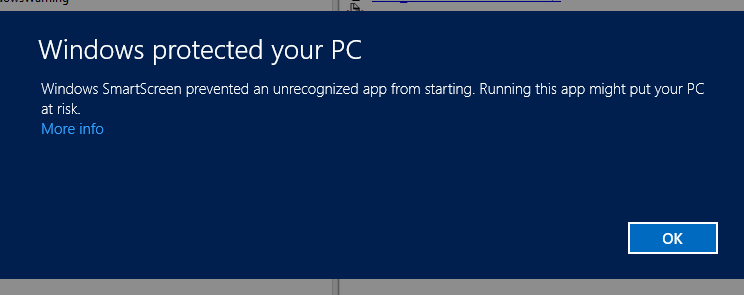
\includegraphics[scale=.5]{windowsWarning.png}
	\caption{Windows 8 warning when trying to run the installer. Select ``More Info'' and then ``Run Anyway.''}
	\label{fig:windowsWarning}
\end{figure}

When the installer file is executed, the installation will begin and show a dialog like the one shown in Figure \ref{fig:windowsInstaller}.  Users should select all options needed:
\begin{itemize}
\item \textbf{hashdb tool}\\
Installs the \hdb tool into the \verb+Program Files+ directory and installs the Users Manual shortcut in the \verb+Start+ menu.
\item \textbf{Add to PATH}\\
Appends the path to the \hdb tool to the System \verb+PATH+ variable so that it can be found at the command prompt and by other tools.
\item \textbf{hashdb Python module}\\
Installs the following files onto the desktop at \verb+Users\Public\Desktop+:
  \begin{itemize}
  \item \verb+hashdb.py+\\
  The \hdb Python interface file.
  \item \verb+_hashdb.pyd+\\
  The \verb+.dll+ file needed by \verb+hashdb.py+.
  \item \verb+test_hashdb_module.py+\\
  A small test program for helping to validate and diagnose the installation of \verb+hashdb.py+ and \verb+hashdb.py+. This file may be delted.
  \end{itemize}

Suggestions for managing these files placed on the public desktop include:
  \begin{itemize}
  \item Move them to your working directory so that they can be found by your Python program.
  \item Move them to another directory and set \verb+PATH+ to include the path to \verb+_hashdb.pyd+ and set \verb+PYTHONPATH+ to include the path to \verb+hashdb.py+.
  \end{itemize}
\end{itemize}

\begin{figure}
	\center
	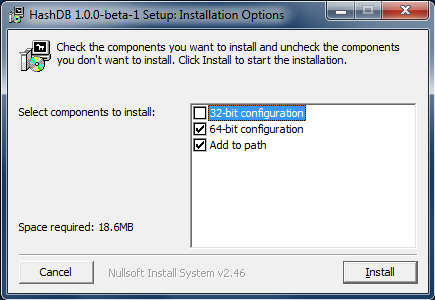
\includegraphics[scale=.8]{WindowsInstaller.png}
	\caption{Dialog appears when the user executes the Windows Installer. Select the default configuration to install all components.}
	\label{fig:windowsInstaller}
\end{figure}

\hdb is now installed on your system can be run from the command line.\\

\subsubsection{Installing on Linux or Mac}
This section describes steps for installing \hdb on a Fedora system and is intended to illustrate the installation process.  For steps on installing \hdb to other flavors of Linux or for MacOS, and for installing specific configurations, please refer to the installation page on the \hdb Wiki at \url{https://github.com/NPS-DEEP/hashdb/wiki/Installing-hashdb}.\\

Before compiling \hdb for your platform, you may need to install other packages on your system which \hdb requires to compile cleanly and with a full set of capabilities.\\

\textbf{Dependencies}\\
The following commands should add the requisite packages:
\begin{Verbatim}[commandchars=\\\{\}]
\verbbf{sudo dnf update}
\verbbf{sudo dnf groupinstall development-tools}
\verbbf{sudo dnf install gcc-c++}
\verbbf{sudo dnf install openssl-devel}
\verbbf{sudo dnf install libewf-devel}
\verbbf{sudo dnf install bzip2-devel}
\verbbf{sudo dnf install swig}
\verbbf{sudo dnf install python-devel}
\end{Verbatim}

\textbf{Download and Install \hdb}\\
Next, download the latest version of \hdb. The software can be downloaded from \url{http://digitalcorpora.org/downloads/hashdb/}. The file to download is \texttt{hashdb-x.y.z.tar.gz} where x.y.z is the latest version.\\

After downloading the file, un-tar it by either right-clicking on the file and choosing ``extract to...' or typing the following at the command line:
\begin{Verbatim}[commandchars=\\\{\}]
\verbbf{tar -xvf hashdb-x.y.z.tar.gz}
\end{Verbatim}

Then, in the newly created \textit{hashdb-x.y.z} directory, run the following commands to install \hdb in \textit{/usr/local/bin} (by default):

\begin{Verbatim}[commandchars=\\\{\}]
\verbbf{./configure}
\verbbf{make}
\verbbf{sudo make install}
\end{Verbatim}
\hdb is now installed on your system and can be run from the command line. \\

Note: sudo is not required. If you do not wish to use sudo,  build and install \hdb in your own space at ``\$HOME/local'' using the following commands:
\begin{Verbatim}[commandchars=\\\{\}]
\verbbf{./configure --prefix=$HOME/local/ --exec-prefix=$HOME/local CPPFLAGS=-}
\textbf{                         I$HOME/local/include/ LDFLAGS=-L$HOME/local/lib/}
\verbbf{make}
\verbbf{make install}
\end{Verbatim}

\textbf{Run \hdb}\\
When installed as administrator, the \hdb tool should automatically be accessible. When installed as a user, the \hdb tool can be made available by typing:
\begin{Verbatim}[commandchars=\\\{\}]
\verbbf{export PATH=$HOME/local/bin:$PATH}
\end{Verbatim}

\textbf{Import the Python \hdb Module}\\
To use the Python \hdb module, your shell must have access to the installed \verb+python.py+ and \verb+_python.so+ resources.\\

When installed as administrator, the \hdb Python interface can be made available by typing:
\begin{Verbatim}[commandchars=\\\{\}]
\verbbf{export PYTHONPATH=/usr/local/lib/python2.7/site-packages:/usr/local/}
\textbf{                         lib64/python2.7/site-packages}
\end{Verbatim}

When installed as a user, the \hdb Python interface can be made available by typing:
\begin{Verbatim}[commandchars=\\\{\}]
\verbbf{export PYTHONPATH=~/local/lib/python2.7/site-packages:~/local/lib64/}
\textbf{                         python2.7/site-packages}
\end{Verbatim}

\subsubsection{Quickstart Guide}
The following steps provide a very brief introduction to running your new installation of \hdb. Steps include creating a demo database and scanning for matching hashes. 
\begin{enumerate}
\item Navigate to the directory where you would like to create a hash database. Then, to run \hdb from the command line, type the following instructions: 
\begin{Verbatim}[commandchars=\\\{\}]
\verbbf{hashdb create demo.hdb}
\end{Verbatim} 

In the above instructions, \texttt{\textbf{demo.hdb}} is the empty database that will be created with default database settings.

\item Next, import data into the database. In this example, lets import hashes from the Kitty Material demo dataset available at \url{http://digitalcorpora.org/corpora/scenarios/2009-m57-patents/KittyMaterial}. But rather than downloading these files and ingesting them, lets just import the pre-made \verb+KittyMaterial.json+ data available at \url{http://digitalcorpora.org/downloads/hashdb/demo/KittyMaterial.json}. After downloading this, type the following:
\begin{Verbatim}[commandchars=\\\{\}]
\verbbf{hashdb import demo.hdb KittyMaterial.json}
\end{Verbatim} 
This command, if executed successfully, will print processing status followed by statistics indicating changes to the database.

\item Next, scan a media image for matching hashes. In this example, lets scan the demo media image available at \url{http://digitalcorpora.org/corpora/scenarios/2009-m57-patents/drives-redacted/jo-favorites-usb-2009-12-11.E01} which contains blacklist block hashes from the Kitty demo:
\begin{Verbatim}[commandchars=\\\{\}]
\verbbf{hashdb scan_media demo.hdb jo-favorites-usb-2009-12-11.E01}
\end{Verbatim} 
With this media and dataset, the first block hash matched is at offset \verb+2543104+ for hash \verb+1d7379fd4d5cf676a9d4de1e48337e71+:

\begingroup
\footnotesize
\begin{Verbatim}[fontfamily=courier]
2543104	1d7379fd4d5cf676a9d4de1e48337e71	{"block_hash":
"1d7379fd4d5cf676a9d4de1e48337e71","k_entropy":4880,
"block_label":"","count":1,"source_list_id":1193146442,"sources":
[{"file_hash":"1dd00f2e51aeebe7541cea4ade2e20b5","filesize":1549288,
"file_type":"","zero_count":0,"nonprobative_count":10,"name_pairs":
["/home/bdallen/KittyMaterial","/home/bdallen/KittyMaterial/
HighQuality/DSC00003.JPG"]}],"source_offsets":
["1dd00f2e51aeebe7541cea4ade2e20b5",1,[0]]}
\end{Verbatim}
\endgroup

\end{enumerate}

\section{How \hdb Works}
The \hdb tool provides capabilities to create, edit, access and search databases of cryptographic hashes created from hash blocks. The cryptographic hashes are imported into a database from a directory, another database, \textbf{bulk\_extractor} or JSON data, or trough the \hdb API.
Once a databases is created, \hdb provides users with the capability to scan the database for matching hash values and identify matching content. Hash databases can be exported, added to, subtracted from and shared.\\


Figure \ref{fig:overviewFigure} provides an overview of the capabilities included with the \hdb tool. \hdb populates databases from whitelist source files
or other media provided in JSON format or through the API.
Users can add or remove data from the database after it is created.
Once the database is populated, \hdb can export content from the database in JSON format. It also provides an API that can be used by third party tools (as it is used in the \bulk program) to create, populate and access hash databases.\\

\begin{figure}
	\center
	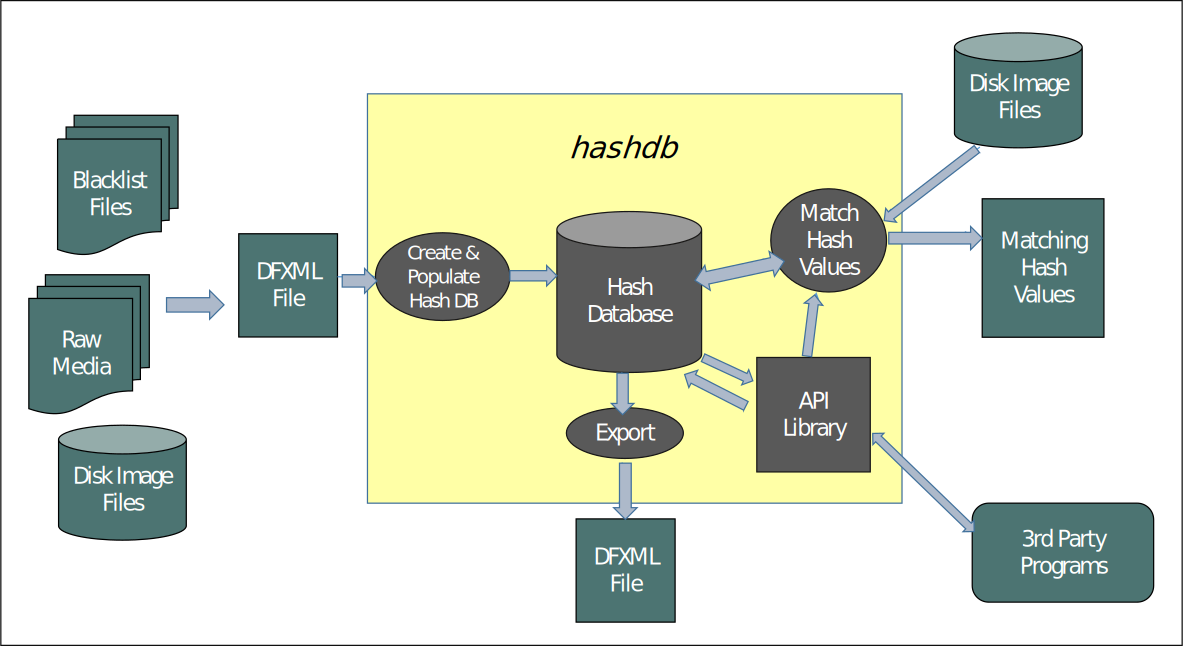
\includegraphics[scale=.45]{drawings/hashdb_system_overview}
	\caption{Overview of the \hdb system}
	\label{fig:overviewFigure}
\end{figure}

\subsection{Block Hash}
\hdb works by matching hashes calculated from blocks of data.  \hdb is different from tools that match files because it can find matches even when part of a file is missing or changed.  \hdb stores and scans for hashes created from contiguous blocks of data.  We call the size of the block hashed the \textit{block size}.  \hdb stores and scans for hashes in step increments along a hash interval. Blocks hashed at step-sized intervals are illustrated in Figure \ref{fig:hashInterval}.\\

\begin{figure}
	\center
	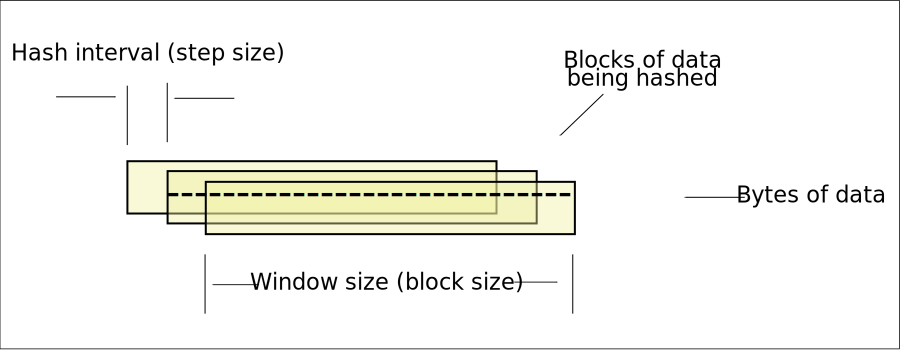
\includegraphics[scale=.45]{drawings/hash_interval}
	\caption{Data blocks are hashed along an interval of bytes}
	\label{fig:hashInterval}
\end{figure}

\begin{figure}
	\center
	
\includegraphics[scale=.45]{drawings/default_hash_interval}
	\caption{By default, hashes are calculated from 512 byte blocks of data along 512 byte intervals and the database uses a byte alignment of 512}
	\label{fig:defaultHashInterval}
\end{figure}

As an optimization, \hdb provides a byte alignment setting. The byte alignment value must be divisible by the step size. The default configuration with 512 for step size, block size, and byte alignment is shown in Figure \ref{fig:defaultHashInterval}. Byte alignment is described in \textbf{\autoref{DBSettings}}.\\

\subsection{Blacklist Data}
Blacklist data is the data we scan against to determine whether forensic data
contains probative artifact.
We build a hash database of blacklist data by importing block hashes
from blacklist files, copying from other hash databases,
or importing from other sources using data prepared in JSON format.\\

Each block hash in the database contains one or more file offsets for one or more sources indicating a source and location within the source where the hash is located.  If a block is found several times for a source, then several offsets will be recorded for that source. If a block is found in more than one source, then more than one source will contain offset information for each source. Block hashes with many source offsets tend to contain non-probative data.\\

\subsection{Repository Names}
Blacklist data may come from multiple sources called ``repositories''. \hdb tracks repository names in order to know what categories blacklist data belongs to. When importing into a database, users may provide repository names specific to balcklist categories or cases, or allow \hdb to select default values.  When scanning, hashes may match sources from several repositories.\\

\subsection{Forensic Data}
Forensic data is the data we scan to see if it contains artifact matching
that in our hash database.
Note that just having matches is not sufficient to be considered probative.
Some matches are common to many files.
\hdb tracks entropy and data information to automate the process
of eliminating many false positives.
Direct analysis such as that provided by the \sscope tool
may be used to see the exact content at that location.
\sscope is available at \url{https://github.com/NPS-DEEP/NPS-SectorScope/wiki}.

\subsection{Recursive Extraction}
The \hdb \verb+ingest+, \verb+scan_media+, and \verb+read_media+ commands support recursive extraction, meaning that they can recursively decompress compressed content. For \verb+ingest+, the result is that compressed source data is uncompressed and submitted as a new file to be ingested. For \verb+scan_media+, the result is that compressed media is recursively uncompressed and scanned. For \verb+read_media+, the media image offset is recursively interpreted and the uncompressed content is returned. \hdb currently decompresses \textbf{zip} and \textbf{gzip} encodings.

\subsection{Recursion Path}
Typically, an offset points directly to a byte in a source file or a media image. But when data is decompressed or recursively decompressed, it includes a recursion path to reach the decompressed data. An offset consists of the following:
\begin{itemize}
\item The byte offset into the data, specifically, a source file or media image.
\item Zero or more recursion path sequences, from out to in, consisting of:
  \begin{itemize}
  \item A delimiter (\textbf{-}).
  \item The uncompression algorithm, such as \textbf{zip}.
  \item A delimiter (\textbf{-}).
  \item The byte offset into the uncompressed data.
  \end{itemize}
\end{itemize}

Example byte offset 2100 at recursion path \verb+1000-zip-2100+ within uncompressed data obtained by unzipping data starting at byte 1000 of file \verb+myfile+ is shown in Figure \ref{fig:recursionPath}.

\begin{figure}
	\center
	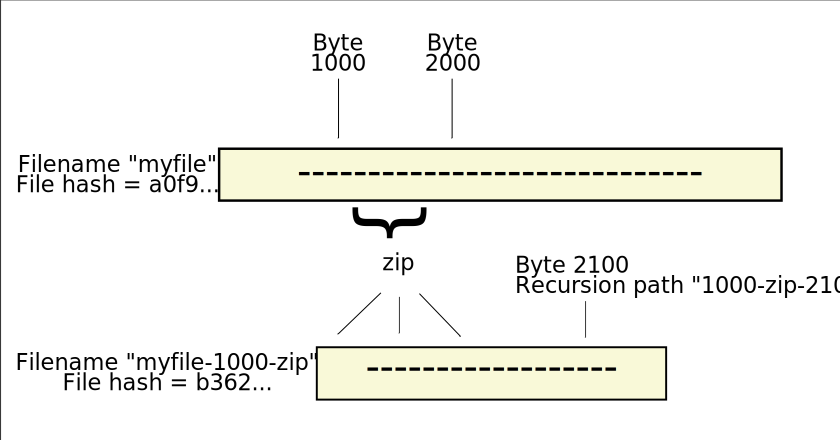
\includegraphics[scale=.45]{drawings/recursion_path}
	\caption{Example of new file \texttt{myfile-100-zip} uncompressed from file \texttt{myfile}}
	\label{fig:recursionPath}
\end{figure}

\subsection{File Hash}
\hdb tracks sources by their file hash rather than by their filename
or repository name.  This approach provides several benefits:

\begin{itemize}
\item The database does not store block hashes from multiple sources
when the sources are actually the same file.
\item Source filenames and repository names for the same file are grouped
together and may be looked up by their file hash value.
\end{itemize}

\subsection{Managing False Positives}
A significant problem when scanning for probative blocks is dealing with false positives \cite{hashBasedCarving}. False positives arise from data that is easily generated or commonly duplicated such as sparse data or lookup tables. \hdb records and uses information about blocks and sources in order to identify blocks as nonprobative. Then, post-processing tools such as \sscope can readily evaluate matched blocks with these false positives removed.\\

Here we describe the data that \hdb stores with hashes and sources. How this data is used to classify blocks as nonprobative is a complex issue. \hdb stores this data. It is up to post-processing tools such as \sscope to evaluate it.\\

Data stored with sources:
\begin{itemize}
\item \textbf{File Hash}\\
Matched source files are indexed by file hash (new to \hdb v3). The \sscope tool uses this value to visualize how specific source files are distributed across a media image.
\item \textbf{File Size}\\
The source file size indicates how big a source file is. The \sscope tool uses this value to know what percentage of a source file is matched in a scan.
\item \textbf{File Type}\\
This field stores information about the type of the source file. This field is not used by the \hdb Tool but is available through the \hdb API interfaces for classifying the file type.
\item \textbf{File Zero Count}\\
The zero count indicates the number of blocks in the source consisting completely of the 0 byte.  These blocks are skipped by the \hdb \verb+scan_stream+ and \verb+ingest+ commands and are not imported into the database or scanned for.
\item \textbf{File Nonprobative Count}\\
The nonprobative count indicates how many blocks of the source file are deemed nonprobative. In the \bulk \hdb scanner import function and in the \hdb tool \verb+ingest+ function, this value is set to the number of blocks that have been given a block label, indicating that the block is likely nonprobative.
\item \textbf{Name Pairs}\\
The name pairs identify the list of all source repository name and filename pairs associated with a source file as identified by the source file hash. When scanning, this list provides a comprehensive indication of what a hash match is a member of.
\end{itemize}
Data stored with hashes:
\begin{itemize}
\item \textbf{Block Hash}\\
The block hash is the hash value calculated from a block of data. \hdb databases are populated with block hash values from sources. When scanning, block hash values are calculated from media images and are scanned for in a \hdb database.
\item \textbf{Entropy}\\
We calculate the entropy of data blocks and use this value to help estimate that the block may be nonprobative. Blocks with a low entropy value are often nonprobative. \hdb calculates the Shannon entropy of blocks using an alphabet of $2^{16}$ values. \hdb provides entropy as \verb+k_entropy+, entropy scaled up by $1,000$ so that it can be managed as an integer. Divide \verb+k_entropy+ by $1,000$ to obtain actual entropy with three decimal place precision.\\

Data in blocks can be a member of many types of alphabets, for example readable text or executable code. For improved results, we recommend considering the type of data along with the calculated entropy when estimating that a block may be nonprobative.
\item \textbf{Block Label}\\
Block labels may be used to hold information about the nature of the block.  For example it might be used to indicate that the byte values increment, indicating a homogeneous data structure \cite{hashBasedCarving}.
\item \textbf{Count}\\
The count indicates the total number of source offsets matching a given block. High count values are likely to be nonprobative.
\item \textbf{Source Offsets}\\
The list of source offset information provides offset information for each source related to the block:
  \begin{itemize}
  \item The \textbf{file hash} of the associated block.
  \item The \textbf{sub-count} of offsets attributed by the given source.
  \item The list of \textbf{file offsets} where the block is found in the given source. Long lists are truncated to conserve space.
  \end{itemize}
\end{itemize}

\subsection{Building a \hdb Database}
There are several ways to populate a database:

\begin{itemize}
\item Using the \hdb \verb+import+ command.
\item Importing from correctly formatted JSON data.
\item Importing from another database.
\item Using the \bulk \hdb scanner.
\item Using the \hdb library through the Python or C++ interface.
\end{itemize}

A database may contain blacklist hashes from multiple source domains,
where a domain is called a \textit{repository}.
The repository name indicates the provenance of the dataset.
It is its description information, such as ``Company X's intellectual property files''.\\

\subsection{Scanning}
There are multiple ways users can scan for matches in a block hash database:

\begin{itemize}
\item Using one of the \hdb tool scan commands to scan from a media image,
list, stream, or specific hash.
\item Using one of the \hdb library Python or C++ scan interfaces.
\item Using the \bulk \hdb scanner Scan function.
\end{itemize}

Additionally, there are several output modes for receiving scan matches. These modes provide varying levels of detail and speed.

\subsection{Contents of a Hash Database}
\label{ContentsOfDB}
Each \hdb database is contained in a directory called \textit{$<$databasename$>$.hdb} and contains a number of files. These files are:

\begingroup
\footnotesize
\begin{Verbatim}[fontfamily=courier]
lmdb_hash_data_store/data.mdb
lmdb_hash_data_store/lock.mdb
lmdb_hash_store/data.mdb
lmdb_hash_store/lock.mdb
lmdb_source_data_store/data.mdb
lmdb_source_data_store/lock.mdb
lmdb_source_id_store/data.mdb
lmdb_source_id_store/lock.mdb
lmdb_source_name_store/data.mdb
lmdb_source_name_store/lock.mdb
log.txt
settings.json
\end{Verbatim}
\endgroup

These files include several data store directories and files, a settings file, and a log file:

\begin{itemize}
\item \texttt{lmdb store} files \\
The \texttt{lmdb store} files encode all the block hashes, source files, and related information that are in the database. These filenames start with the prefix \verb+lmdb+.

\item \texttt{settings.json} \\
This file contains the settings requested by the user when the block hash database was created. Database settings are described in \textbf{\autoref{DBSettings}}. This file also contains the internal \hdb settings version used to help \hdb identify whether a database is compatible with this version of \hdb. The \texttt{settings.json} file with the default settings looks like this:

\begingroup
\footnotesize
\begin{Verbatim}[fontfamily=courier]
{"settings_version":3, "byte_alignment":512, "block_size":512,
"hash_prefix_bits":28, "hash_suffix_bytes":3}
\end{Verbatim}
\endgroup

\item \texttt{log.txt} \\
Every time a command is run that changes the content of the database, information about the change is appended to this log.  Each entry includes the command name, information about \hdb including the command typed and how \hdb was compiled, information about the operating system \hdb was just run on, timestamps indicating how much time the command took, and the specific \hdb changes applied.\\

Listing \ref{logfile} shows an example log file containing two entries, one for when the hash database was created, and one for when data was ingested into the database.

\lstset{style=customfile}
\begin{lstlisting}[float, caption=An example \texttt{log.xml} log file showing a database creation entry and a datase ingest entry, label=logfile]
# command: "hashdb create KittyMaterial.hdb"
# hashdb version: 3.0.0-alpha-9
# username: bdallen
# start time 2016-09-08T22:57:49Z
{"name":"begin","delta":"0.000365","total":"0.000365"}
{"name":"end","delta":"0.000018","total":"0.000392"}
# command: "hashdb ingest KittyMaterial.hdb ../KittyMaterial"
# hashdb version: 3.0.0-alpha-9
# username: bdallen
# start time 2016-09-08T22:58:07Z
{"name":"begin","delta":"0.000326","total":"0.000326"}
# hashdb changes:
#     hash_data_source_inserted: 401713
#     hash_data_offset_inserted: 401732
#     hash_prefix_inserted: 401316
#     hash_suffix_inserted: 401598
#     hash_count_changed: 88
#     hash_not_changed: 46
#     source_data_inserted: 88
#     source_data_changed: 88
#     source_id_inserted: 88
#     source_id_already_present: 401820
#     source_name_inserted: 88
{"name":"end","delta":"9.397511","total":"9.397846"}
\end{lstlisting}


\item \texttt{timestamp.json}\\
\verb+timestamp.json+ is not formally part of the \hdb database.  It is created by the \hdb tool performance analysis commands described in \textbf{\autoref{PerformanceAnalysis}}. This file is replaced rather than appended to. Timestamp syntax is described in \textbf{\Autoref{InputOutputSyntax}}.
\end{itemize}

\subsection{Database Settings}
\label{DBSettings}
Function and performance of a \hdb database is set using configurable settings:

\begin{itemize}
\item \textbf{Byte alignment}\\
Byte alignment is an optimization parameter created to help reduce the size of the database. To be optimal, this value should be large, but it must be divisible by the step size used when importing hashes. If you only scan storage devices, use the sector size of the storage device since this is the smallest value that data in storage devices can align to, specifically, 512.

\item \textbf{Block size}\\
The size of data blocks the database expects to store. Block hashes are calculated from data of this size. The default is 512.

\item \textbf{Hash prefix bits}\\
The number of bits of the hash prefix to use as the key in the store. The idea is to select a value given the size of the database so that the average number of hashes with this prefix is slightly greater than 0, for example 20. For example if you expect 5 billion hashes, you might select 28 because $5/2^{28}=18.6$, which is near 20.

\item \textbf{Hash suffix bytes}\\
The number of bytes of the hash suffix to store in the set of values of hash suffixes for this hash key. The idea is to store as few bytes as possible while minimizing false positives. For example if you expect 5 billion hashes, you might select 28 prefix bits and 3 suffix bytes because $5 / 2^{((28) + 8*(3))} = 5 / 2^{52} = 0.00011\%$ false positive rate, about 1 in 1 million.
\end{itemize}

\subsection{Maintaining Database Integrity}
A \hdb hash database can be damaged when operations that modify it are aborted. Re-running the operation may not fully add missing data. Although some data may be lost, the database should remain operational.\\

A \hdb hash database can also be damaged by running a command that should not have been run such as ingesting incorrect files or adding an incorrect database. Some operations can be ``rolled out'' using database manipulation commands.\\

Each \hdb hash database includes an audit log file that records all commands issued that modify that database. You may inspect this audit log to verify that all issued commands are acceptable and that all issued commands have completed. Audit log files are described in \textbf{\autoref{ContentsOfDB}}.\\

Please backup databases that cannot readily be recreated.

\section {Running the \hdb Tool}
\label{Running}
The core capabilities provided by \hdb involve creating and maintaining a database of hash values and scanning media for those hash values. To perform those tasks, \hdb users need to start by building a database (if an existing database is not available for use).
Users then import hashes using \hdb tool commands, the \hdb \bulk scanner, or through the \hdb library API, and then possibly merge or subtract hashes to obtain the desired set of hashes to scan against.
Users then scan for hashes that match.
Additional commands are provided to support statistical analysis, performance tuning and performance analysis.\\

This section describes use of the \hdb tool commands, along with examples, for performing these tasks.
For more examples of command usage, please see \textbf{\autoref{UseCases}}.
For a \hdb quick reference summary, please see \textbf{\autoref{QuickReference}}, also available at \url{http://digitalcorpora.org/downloads/hashdb/hashdb_quick_reference.pdf}.

\subsection{Creating a New Hash Database}
\label{Creating}
A hash database must be created before hashes can be added to it.
Syntax for creating a hash database is shown in Table \ref{tab:createDatabase}.
Configurable settings associated with the database is shown in Table \ref{tab:hashDBSettings} and described in \textbf{\Autoref{DBSettings}}.\\
\begin{table}[!ht]
\centering
\caption{Command for Creating Hash Databases}
\label{tab:createDatabase}
\begin{tabular}{|p{2.5 cm}|p{7 cm}|p{4 cm}|}
\hline \hline
\textbf{Command} & \textbf{Usage} & \textbf{Description} \\
\hline
\textbf{create} & \verb+create [-b <block size>]+ \verb+<hashdb.hdb>+ & Creates a new hash database.\\
\hline
\end{tabular}
\end{table}

\begin{table}[!ht]
\centering
\caption{Database Settings}
\label{tab:hashDBSettings}
\begin{tabular}{|p{1.5 cm}|p{8 cm}|p{4 cm}|}
\hline \hline
\textbf{Option} & \textbf{Verbose Option} & \textbf{Specification} \\
\hline
\textbf{\texttt{-b}} & \verb+--block_size=+\textit{block\_size} & Specifies the block size in bytes used to generate the hashes that will be stored and scanned against. Default is 512 bytes.  \\
\hline
\end{tabular}
\end{table}

\subsubsection{\texttt{create}}
Create a new hash database configured with provided or default settings.\\

\textbf{Example}\\
To create an (empty) hash database named \textbf{\texttt{demo.hdb}}, type the following command:
\begin{Verbatim}[commandchars=\\\{\}]
\verbbf{hashdb create demo.hdb}
\end{Verbatim}
The above command will create a database with all of the default hash database settings. Most users will not need to change these settings.
Users can specify either the option and value or the verbose option value for each parameter along with the create command, as in:\\
\begin{Verbatim}[commandchars=\\\{\}]
\verbbf{hashdb create --block\_size=4096 demo.hdb}
\verbbf{hashdb create -b 4096 demo.hdb}
\end{Verbatim}
The above two commands produce identical results, creating the database \texttt{demo.hdb} to expect a block size of 4096 bytes.\\

\subsection{Importing and Exporting}
Hash databases may be imported to in several ways.  Syntax for commands that import and export hashes is shown in Table \ref{tab:importExport}. Import and export options are shown in Table \ref{tab:ImportExportOptions}.\\

Note that there are other ways to populate a database besides these listed here, including using other hash databases (discussed in \textbf{\autoref{updateSection}}),
by using the \bulk \hdb scanner (discussed in \textbf{\autoref{bulkextractorSection}}),
and through the use of the import capability provided by the \hdb library API (discussed in \textbf{\autoref{APISection}}).\\

\begin{table}[!ht]
\centering
\caption{Commands for Importing into and Exporting Hash Databases}
\label{tab:importExport}
\begin{tabular}{|p{2.5 cm}|p{7 cm}|p{4 cm}|}
\hline \hline
\textbf{Command} & \textbf{Usage} & \textbf{Description} \\
\hline
\textbf{ingest} & \verb+ingest [-r <repository name>]+ \verb+[-w <whitelist.hdb>]+ \verb+[-s <step size>] [-x <rel>]+ \verb+ <hashdb.hdb> <source directory>+& Computes and ingests block hashes from files under the source directory into the hash database as directed by options.\\
\hline
\textbf{import\_tab} & \verb+import_tab [-r <repository name>]+ \verb+<hashdb.hdb>+ \verb+<tab.txt>+& Imports values from the tab-delimited file into the hash database. This command accepts a dash (\verb+-+) as a filename to allow terminal streaming from \verb+stdin+.\\
\hline
\textbf{import} & \verb+import <hashdb.hdb>+ \verb+<hashdb.json>+& Imports values from the JSON file into the hash database. This command accepts a dash (\verb+-+) as a filename to allow terminal streaming from \verb+stdin+.\\
\hline
\textbf{export} & \verb+export [-p <begin:end>] <hashdb.hdb>+ \verb+<hashdb.json>+& Exports the hash database to the JSON file. This command accepts a dash (\verb+-+) as a filename to allow terminal streaming to \verb+stdout+.\\
\hline
\end{tabular}
\end{table}

\begin{table}[!ht]
\centering
\caption{Options for Importing and Exporting Hash Databases}
\label{tab:ImportExportOptions}
\begin{tabular}{|p{1.5 cm}|p{8 cm}|p{4 cm}|}
\hline \hline
\textbf{Option} & \textbf{Verbose Option} & \textbf{Specification} \\
\hline
\textbf{\texttt{-r}} & \verb+--repository_name=+\textit{repository name} & Specifies the name to associate the imported hashes with. If not provided, the source filename entered is used as the repository name.\\
\hline
\textbf{\texttt{-w}} & \verb+--whitelist_dir=+\textit{whitelist directory} & If a whitelist database is provided, matching hashes are marked with \verb+w+ in their block label.\\
\hline
\textbf{\texttt{-s}} & \verb+--step_size=+\textit{step size} & The increment to step along for calculating block hashes. The step size must be compatible with the byte alignment defined in the database, specifically the byte alignment must be divisible by the byte alignment.\\
\hline
\textbf{\texttt{-x}} & \verb+--disable_processing=rel+ & Use this option to disable specific processing, specifically: \verb+r+ disables recursively processing embedded data, \verb+e+ disables calculating block entropy, and \verb+l+ disables calculating block labels.\\
\hline
\textbf{\texttt{-p}} & \verb+--part_range=+\textit{begin:end} & Use this option to select a range of block hashes by hexadecimal value rather than selecting all block hashes.\\
\hline
\end{tabular}
\end{table}

\subsubsection{\texttt{ingest}}
The \verb+ingest+ command computes and ingests hashes from files under the source directory, including files in subdirectories. Files with \verb+.E01+ extensions are treated as E01 files. If some of the content to be ingested already exists, specifically, if block hashes have already been ingested for a given file hash, it will not be ingested again, but the filename and repository name will be stored to cite the source reference.\\

\textbf{Example}\\
To import block hashes from a directory of blacklist sources, type the following command:
\begin{Verbatim}[commandchars=\\\{\}]
\verbbf{hashdb ingest -r demo_repository demo.hdb demo_blacklist_dir}
\end{Verbatim}
In the above command the option \textbf{-r} is used along with the repository name \texttt{demo\_repository} to indicate the repository source of the block hashes being imported into the database. The repository name is used to keep track of the sources of hashes. By default, the repository name used is the text \texttt{repository\_} with the filename of the file being imported from appended after it.\\

The \textbf{ingest} command in the above example imports block hashes from files in the \texttt{demo\_blacklist\_dir} directory into the database \texttt{demo.hdb}. When the Kitty Material demo dataset available at \url{http://digitalcorpora.org/corpora/scenarios/2009-m57-patents/KittyMaterial/import} is imported, \hdb prints output to the command line to indicate that hashes have been inserted into database \texttt{\textbf{demo.hdb}}. Listing \ref{DatabaseChanges} shows an example output of changes from running an ingest command.\\

Also, database log file \texttt{log.txt} is updated to show that a set of hash blocks have just been inserted. The log in Figure \ref{logfile} was generated from similar \textbf{create} and \textbf{import} actions.  The contents of log files is described in \textbf{\autoref{ContentsOfDB}}.\\

Users may prefer to run statistical commands such as this to get information about the contents of the database (and confirm that values were inserted):
\begin{Verbatim}[commandchars=\\\{\}]
\verbbf{hashdb size demo.hdb}
\end{Verbatim}

\subsubsection{\texttt{import\_tab}}
The \verb+import_tab+ command imports values from the tab-delimited file into the hash database. Note that tab-delimited files are expected to contain block hashes calculated from 512-byte blocks along 512-byte boundaries. Tab-delimited files are described in \textbf{\autoref{TabFile}}.\\

\hdb checks to see if the source file has already been imported and does not import block hashes from sources imported in previous sessions.\\

\subsubsection{\texttt{import}}
The \verb+import+ command imports values from an exported database. Data is in JSON format as described in \textbf{\autoref{ImportExportSyntax}}. If source information for a block hash is already present, it will not be re-imported.

\subsubsection{\texttt{export}}
The \verb+export+ command exports values or a range of values from a \hdb block hash database. Data is in JSON format as described in \textbf{\autoref{ImportExportSyntax}}. The following example exports everything in database \verb+demo.hdb+ to file, \verb+demo.json+:
\begin{Verbatim}[commandchars=\\\{\}]
\verbbf{hashdb export demo.hdb demo.json}
\end{Verbatim}

This example exports everything in database \verb+demo.hdb+ in two parts:
\begin{Verbatim}[commandchars=\\\{\}]
\verbbf{hashdb export -p 00:80 demo.hdb demo_part_1.json}
\verbbf{hashdb export -p 80:ffffffffffffffffffffffffffffffff demo.hdb demo_part_2.json}
\end{Verbatim}

\subsection{Database Manipulation}
\label{DatabaseManipulation}
Databases may need to be merged together or common hash values may need to be subtracted out in order to produce a specific set of blacklist data to scan against.
Syntax for commands that manipulate hash databases is shown in Table \ref{tab:databaseManipulation}.
Destination databases are created if they do not exist yet.
\begin{table}[!ht]
\centering
\caption{Commands to Manipulate Hash Databases}
\label{tab:databaseManipulation}
\begin{tabular}{|p{3.5 cm}|p{6 cm}|p{4 cm}|}
\hline \hline
\textbf{Command} & \textbf{Usage} & \textbf{Description} \\
\hline
\textbf{add} & \verb+add <source db>+ \verb+<destination db>+ & Copies all of the hashes from \textit{source db} to \textit{destination db}\\
\hline
\textbf{add\_multiple} &  \verb+add_multiple <source db1>+ \verb+<source db2> ...+ \verb+<destination db>+ & Adds databases \textit{source db1}, \textit{source db2}, etc.\ to \textit{destination db}\\
\hline
\textbf{add\_repository} & \verb+add_repository <source db>+ \verb+<destination db>+ \verb+<repository name>+ & Adds \textit{source db} to \textit{destination db} but only when the repository name matches\\
\hline
\textbf{add\_range} & \verb+add_range<source db>+ \verb+<destination db>+ \verb+<m:n>+&   Copies hash values from \textit{source db} into \textit{destination db} that have source counts within range $m$ and $n$, inclusive\\
\hline
\textbf{intersect} & \verb+intersect <source db1>+ \verb+<source db2> <destination db>+ &   Copies hash values common to both \textit{source db1} and \textit{source db2} into \textit{destination db} where sources match\\
\hline
\textbf{intersect\_hash} & \verb+intersect_hash <source db1>+ \verb+<source db2> <destination db>+ &   Copies hash values common to both \textit{source db1} and \textit{source db2} into \textit{destination db} even if their sources are different.\\
\hline
\textbf{subtract} & \verb+subtract <source db1>+ \verb+<source db2> <destination db>+&   Copies hash values found in \textit{source db1} but not in \textit{source db2} into \textit{destination db} where sources match\\
\hline
\textbf{subtract\_hash} & \verb+subtract <source db1>+ \verb+<source db2> <destination db>+&   Copies hash values found in \textit{source db1} but not in \textit{source db2} into \textit{destination db} even if their sources are different.\\
\hline
\textbf{subtract \_repository} & \verb+subtract_repository+ \verb+<source db1>+ \verb+<destination db2>+ \verb+<repository namedb>+ & Adds \textit{source db1} to \textit{destination db2} unless the repository name matches\\
\hline
\end{tabular}
\end{table}

\subsubsection{\texttt{add}}
Add a database to another database.
\subsubsection{\texttt{add\_multiple}}
Add multiple databases into a destination database. This can be faster than using add multiple times because the destination is built in lexicographical order.
\subsubsection{\texttt{add\_repository}}
Add a database to another database but only when the repository name matches. Use this to copy everything belonging to a repository to a new database.
\subsubsection{\texttt{add\_range}}
Add a database to another database but only when the hash source count falls within the given range. Use this to isolate hashes that appear with a certain frequency or to remove hashes that are too popular.
\subsubsection{\texttt{intersect}}
Add hashes to a destination database when the hash and source are common. Use this to find the intersection between two databases.
\subsubsection{\texttt{intersect\_hash}}
Add hashes to a destination database when the hash is common, even if the referenced sources are different. Use this to find hashes that intersect between two databases even if their sources do not intersect.
\subsubsection{\texttt{subtract}}
Add hashes to a destination database when the hash and source is in the first database but not in the second. Use this to ensure that hashes in the second database do not appear in the new destination database.
\subsubsection{\texttt{subtract\_hash}}
Add hashes to a destination database when the hash is in the first database but not in the second, even if the referenced sources are different. Use this to ensure that hashes in the second database do not appear in the new destination database even when the sources are different.
\subsubsection{\texttt{subtract\_repository}}
Add a database to another database but only when the repository name does not match. Use this to ensure that hashes in the new destination database do not include the repository being subtracted. If information is also contributed from another repository, the information will still be copied but the reference to the removed repository will not be copied.

\subsection{Scan Services}
\label{ScanServices}
\hdb can be used to determine if a file, directory or media image has content that matches previously identified content. This capability can be used, for example, to determine if a set of files contains a specific file excerpt or if a media image contains a video fragment. Forensic investigators can use this feature to search for blacklisted content.
Syntax for scan service commands is shown in Table \ref{tab:scanServices}. Scan service options are shown in Table \ref{tab:ScanOptions}.\\

\begin{table}[!ht]
\centering
\caption{Commands that Provide Scan Services}
\label{tab:scanServices}
\begin{tabular}{|p{3.5 cm}|p{6 cm}|p{4 cm}|}
\hline \hline
\textbf{Command} & \textbf{Usage} & \textbf{Description} \\
\hline
\textbf{scan\_list} & \verb+scan_list [-j e|o|c|a] <hashdb>+ \verb+<hash list file>+ & Scans the hashdb for hashes that match hashes in the hash list file and prints out matches\\
\hline
\textbf{scan\_hash} & \verb+scan_hash [-j e|o|c|a] <hashdb>+ \verb+<hash value>+ & Scans the hashdb for the specified hash value and prints out whether it matches\\
\hline
\textbf{scan\_media} & \verb+scan_media+ \verb+[-s <step size>] [-j e|o|c|a]+ \verb+[-x <r>] <hashdb> <media media>+ & Scans the hashdb for hashes that match hashes in the media image and prints out matches.\\
\hline
\end{tabular}
\end{table}

\begin{table}[!ht]
\centering
\caption{Options for Scanning from a Media Image}
\label{tab:ScanOptions}
\begin{tabular}{|p{1.5 cm}|p{8 cm}|p{4 cm}|}
\hline \hline
\textbf{Option} & \textbf{Verbose Option} & \textbf{Specification} \\
\hline
\textbf{\texttt{-s}} & \verb+--step_size=+\textit{step size} & The increment to step along for calculating block hashes. The step size must be compatible with the byte alignment defined in the database, specifically the byte alignment must be divisible by the byte alignment.\\
\hline
\textbf{\texttt{-j}} & \verb+--json_scan_mode=e|o|c|a+ & Select a mode, one of \textbf{e}xpanded, expanded \textbf{o}ptimized, \textbf{c}ount only, \textbf{a}pproximate count. Default is \textbf{o}.\\
\hline
\textbf{\texttt{-x}} & \verb+--disable_processing=r+ & Use this option to disable specific processing, specifically: \verb+r+ disables recursively processing embedded data.\\
\hline
\end{tabular}
\end{table}

\subsubsection{\texttt{scan\_list}}
Scan for hashes in the list of hashes. List input syntax is described in \textbf{\autoref{ScanListInputFile}}. Scan output is described in \textbf{\autoref{ScanData}}. This command accepts a dash (\verb+-+) as a filename to allow terminal streaming from \verb+stdin+.\\
\subsubsection{\texttt{scan\_hash}}
Scan for the specified hash. The hash to scan for must be provided in hexadecimal format.
\subsubsection{\texttt{scan\_media}}
Scan the specified media image for matching hashes.\\

\textbf{Example}\\
To scan, first identify the media that you would like to scan. For this example, we download and use the demo media image available at \url{ http://digitalcorpora.org/corpora/scenarios/2009-m57-patents/drives-redacted/jo-favorites-usb-2009-12-11.E01} which contains matching Kitty material.\\

Then identify the existing hash database that will be used to search for hash value matches. We'll use the database \texttt{\textbf{demo.hdb}} that we created from Kitty material in the previous section, containing block hash values calculated from pictures and videos of cats.\\

Finally, run the \hdb scan command to scan for blocks in the media that match block hashes in the database:
\begin{Verbatim}[commandchars=\\\{\}]
\verbbf{hashdb scan_media demo.hdb jo-favorites-usb-2009-12-11.E01 > matches.json}
\end{Verbatim}
This command tells \hdb to scan media image \verb+jo-favorites-usb-2009-12-11.E01+ and try to match the values found in the local database \texttt{\textbf{demo.hdb}}, putting match data in file \verb+matches.json+.  An example match might look like this:

\begingroup
\footnotesize
\begin{Verbatim}[fontfamily=courier]
2543104	1d7379fd4d5cf676a9d4de1e48337e71	{"block_hash":
"1d7379fd4d5cf676a9d4de1e48337e71","k_entropy":4880,
"block_label":"","count":1,"source_list_id":1193146442,"sources":
[{"file_hash":"1dd00f2e51aeebe7541cea4ade2e20b5","filesize":1549288,
"file_type":"","zero_count":0,"nonprobative_count":10,"name_pairs":
["/home/bdallen/KittyMaterial","/home/bdallen/KittyMaterial/
HighQuality/DSC00003.JPG"]}],"source_offsets":
["1dd00f2e51aeebe7541cea4ade2e20b5",1,[0]]}
\end{Verbatim}
\endgroup

Users may be put off by the quantity of matches incurred by low-entropy data in their databases such as number tables or metadata header blocks from files that are otherwise unique. Database manipulation commands,
\textbf{\autoref{DatabaseManipulation}}, can mitigate this, for example:
\begin{itemize}
\item Use the ``subtract'' command to remove known whitelist data created from sources such as ``brand new'' operating system media images and the NSRL.
\item Alternatively, use the ``add\_range'' command to copy all hash values that have been imported some number of times, for example, exactly once.
\end{itemize}

\subsection{Statistics}
Various statistics are available about a given hash database including the size of a database, where its hashes were sourced from, a histogram of its hashes, and more.
Table \ref{tab:statistics} shows syntax for the statistics commands.
Statistics options are shown in Table \ref{tab:StatisticsOptions}.
\begin{table}[!ht]
\centering
\caption{Commands that provide Statistics about Hash Databases}
\label{tab:statistics}
\begin{tabular}{|p{3.5 cm}|p{6 cm}|p{4 cm}|}
\hline \hline
\textbf{Command} & \textbf{Usage} & \textbf{Description} \\
\hline
\textbf{size} & \verb+size <hashdb>+ & Prints out size information relating to the database.\\
\hline
\textbf{sources} & \verb+sources <hashdb>+ & Prints source information for all sources in the database.\\
\hline
\textbf{histogram} & \verb+histogram <hashdb>+ & Prints a hash distribution for the hashes in the \textit{hashdb}.\\
\hline
\textbf{duplicates} & \verb+duplicates <hashdb> <number>+ &  Prints out hashes in the database that are sourced the given number of times.\\
\hline
\textbf{hash\_table} & \verb+hash_table <hashdb>+ \verb+<hex file hash>+ &  Prints hashes associated with the specified source.\\
\hline
\textbf{read\_media} & \verb+read_media <media image file>+ \verb+<offset> <count>+ &  Prints count raw bytes from a media image file starting at the given offset.\\
\hline
\end{tabular}
\end{table}

\begin{table}[!ht]
\centering
\caption{Options for Commands that Provide Statistics}
\label{tab:StatisticsOptions}
\begin{tabular}{|p{1.5 cm}|p{8 cm}|p{4 cm}|}
\hline \hline
\textbf{Option} & \textbf{Verbose Option} & \textbf{Specification} \\
\hline
\textbf{\texttt{-j}} & \verb+--json_scan_mode=e|o|c|a+ & Select a mode, one of \textbf{e}xpanded, expanded \textbf{o}ptimized, \textbf{c}ount only, \textbf{a}pproximate count. Default is \textbf{o}.\\
\hline
\end{tabular}
\end{table}

\subsubsection{\texttt{size}}
Prints size information about the given database. Size values are specific to the underlying database storage implementation and indicate how large the parts of the database are.\\

To find the size of various data stores in hash database \texttt{example.hdb},
type the following:
\begin{Verbatim}[commandchars=\\\{\}]
\verbbf{hashdb size examle.hdb}
\end{Verbatim}
The above command prints the size of various data stores within the database in JSON format.

\subsubsection{\texttt{sources}}
Prints out all source file references that have contributed to this database including repository names and filenames.

\subsubsection{\texttt{histogram}}
Prints a hash distribution of the hashes in the given database, see \textbf{\autoref{Histogram}} for output syntax.

\subsubsection{\texttt{duplicates}}

Prints out hashes in the database that are sourced the given number of times.
\subsubsection{\texttt{hash\_table}}
Prints out hashes associated with the specified source identified by the source file hexdigest.

To obtain a list of hashes in \texttt{example.hdb} associated with the source file identified by hexcode \texttt{16d75027533b0a5ab900089a244384a0}, type the following:
\begin{Verbatim}[commandchars=\\\{\}]
\verbbf{hashdb hash_table example.hdb 16d75027533b0a5ab900089a244384a0}
\end{Verbatim}

\subsubsection{\texttt{read\_media}}
Prints raw bytes from the given media image. Note that these bytes are often not printable.

\subsection{Performance Analysis}
\label{PerformanceAnalysis}
Performance analysis commands for analyzing \hdb performance are shown in Table \ref{tab:analysis}. Performance analysis options are shown in Table \ref{tab:AnalysisOptions}. Timing data is placed in file \verb+timestamp.json+, replacing any previous content.

\begin{table}[!ht]
\centering
\caption{Commands that Support \hdb Performance Analysis}
\label{tab:analysis}
\begin{tabular}{|p{3.5 cm}|p{6 cm}|p{4 cm}|}
\hline \hline
\textbf{Command} & \textbf{Usage} & \textbf{Description} \\
\hline
\textbf{add\_random} & \verb+add_random+ \verb+-r [<repository name>]+ \verb+<hashdb.hdb> <count>+ & Adds count random hashes to the given database, creating timing data in the \texttt{log.xml} file.\\
\hline
\textbf{scan\_random} & \verb+scan_random [-j e|o|c|a]+ \verb+<hashdb.hdb>+ & Scans random hashes in the given database, creating timing data in the \texttt{log.xml} file.\\
\hline
\textbf{add\_same} & \verb+add_same+ \verb+-r [<repository name>]+ \verb+<hashdb.hdb> <count>+ & Adds count same hashes to the given database, creating timing data in the \texttt{log.xml} file.\\
\hline
\textbf{scan\_same} & \verb+scan_same [-j e|o|c|a]+ \verb+<hashdb.hdb>+ & Scans count same hashes in the given database, creating timing data in the \texttt{log.xml} file.\\
\hline
\end{tabular}
\end{table}

\begin{table}[!ht]
\centering
\caption{Options for Commands that Support Performance Analysis}
\label{tab:AnalysisOptions}
\begin{tabular}{|p{1.5 cm}|p{8 cm}|p{4 cm}|}
\hline \hline
\textbf{Option} & \textbf{Verbose Option} & \textbf{Specification} \\
\hline
\textbf{\texttt{-j}} & \verb+--json_scan_mode=e|o|c|a+ & Select a mode, one of \textbf{e}xpanded, expanded \textbf{o}ptimized, \textbf{c}ount only, \textbf{a}pproximate count. Default is \textbf{o}.\\
\hline
\end{tabular}
\end{table}

\subsubsection{\texttt{add\_random}}
Add random hashes, leaving timing data in \verb+log.xml+.
\subsubsection{\texttt{scan\_random}}
Scan random hashes, leaving timing data in \verb+log.xml+. Although this command does not produce output, the scan mode used impacts timing.
\subsubsection{\texttt{add\_same}}
Add the same hash, leaving timing data in \verb+log.xml+.
\subsubsection{\texttt{scan\_same}}
Scan the same hash, leaving timing data in \verb+log.xml+. Although this command does not produce output, the scan mode used impacts timing.

\section{Tools that use \hdb}
\label{OtherTools}
\sscope, the \sscope Autopsy Plug-in, and the \bulk \hdb scanner use \hdb.

\subsection{\sscope}
The \sscope tool provides a GUI for analyzing data associated with block hash matches found on a media image. An example screenshot of the main window of \sscope showing a histogram of matches on a media image is shown in Figure \ref{fig:SectorScope_main}. \sscope also provides interfaces for building and scanning against \hdb databases. Please see \url{https://github.com/NPS-DEEP/NPS-SectorScope/wiki} for more information on \sscope.

\begin{figure}
	\center
	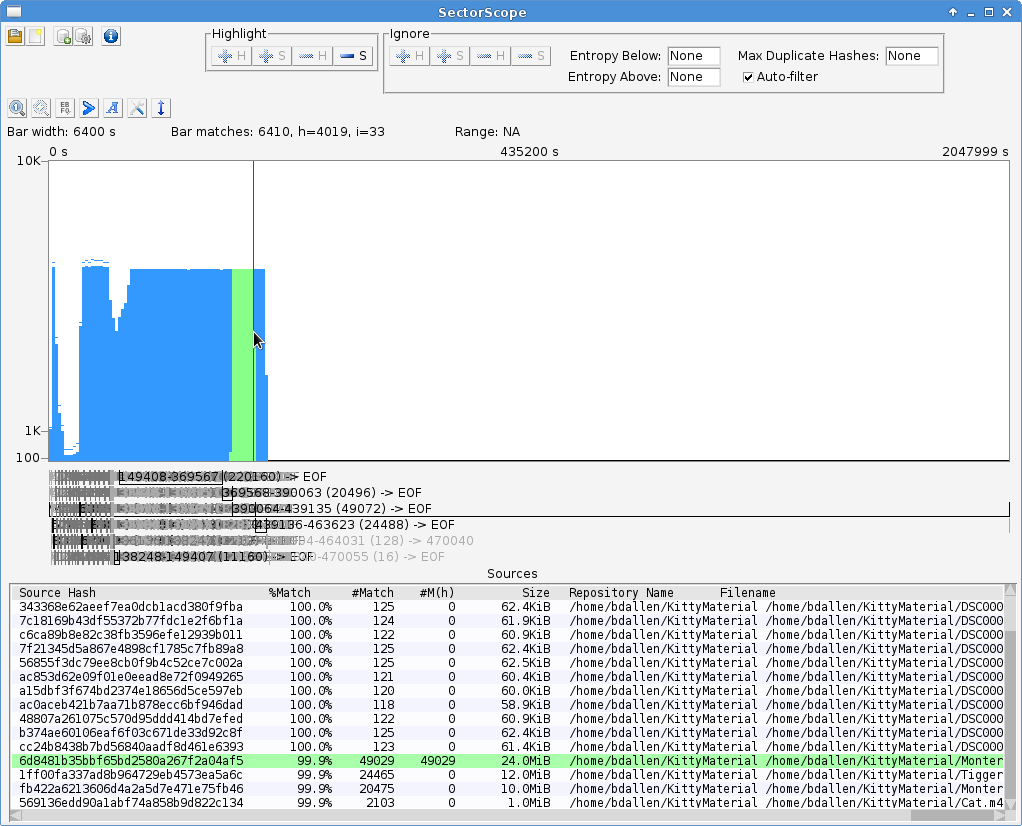
\includegraphics[scale=.45]{drawings/SectorScope_main}
	\caption{Example screenshot of the \sscope tool}
	\label{fig:SectorScope_main}
\end{figure}

\subsection{The \sscope \aut Plug-in}
\sscope provides an \aut plug-in for scanning for fragments of previously identified files. \aut is currently only available on Windows systems. This section describes how to set up the \sscope \aut plug-in.

\subsubsection{Installing the \sscope Plug-in}
The \sscope Windows installer installs the requisite \verb+.nbm+ Autopsy plug-in module onto the desktop. Please follow these steps to install this module:

\begin{enumerate}
\item Open \aut. From the Autopsy menu, select \verb+Tools | Plugins+.
\item Open the \verb+Downloaded+ tab and click the \verb+Add Plugins...+ button.
\item From the \verb+Add Plugins+ window, navigate to the \verb+.nbm+ module file that was installed onto the desktop, and open it.
\item Click \verb+Install+ and follow the wizard. Please note that it may be difficult to replace an old module of NPS-Autopsy-hashdb already installed in Autopsy. In the unlikely case that error \verb+Some plugins require plugin org.jdesktop.beansbinding+ \verb+to be installed+ appears, it may be necessary to uninstall and reinstall Autopsy.
\end{enumerate}

\subsubsection{Configuring the \sscope Plug-in}
The path to the \hdb database to scan against must be configured:

\begin{enumerate}
\item Start a new case, \verb+File | New Case...+, fill in the Case Information fields, and click \verb+Next+.
\item Fill in Case Information and click \verb+Finish+.
\item For Add Data Source (1 of 3), put in a media image for Autopsy to process and click \verb+Next+.
\item For Add Data Source (2 of 3), select checkboxes as desired, then click on \verb+NPS-SectorScope+ text to configure the path to your \hdb database to scan against. Currently a file chooser is not available, so please type in the full path, for example: \verb+C:\Users\me\my_hashdb.hdb+. Click Next.
\item For Add Data Source (3 of 3) click \verb+Finish+. When the NPS-SectorScope module begins processing, Autopsy will display "NPS-SectorScope ..." as \bulk runs, which may take up to several hours. Unfortunately, \bulk progress is not currently indicated. For diagnostics: please see if progress text is appearing in the generated \verb+bulk_extractor\report.xml+ file and in the generated log file or try running the scan manually.
\end{enumerate}

\subsection{\bulk}
\bulk is an open source digital forensics tool that extracts features such as email addresses, credit card numbers, URLs and other types of information from digital evidence files. It operates on disk media images, files or a directory of files and extracts useful information without parsing the file system or file system structures.  For more information on how to use \bulk for a wide variety of applications, refer to the separate publication \textit{The \bulk Users Manual} available at \url{http://digitalcorpora.org/downloads/bulk_extractor/BEUsersManual.pdf} \cite{beusersguide}.\\

In particular, a \hdb \bulk scanner is available which may be used to import block hashes into a new hash database and to scan for hashes against an existing hash database.
Currently, \hdb requires a newer build of \bulk than is available on the \bulk site.
Please see the \hdb Wiki page at \url{https://github.com/NPS-DEEP/hashdb/wiki}
for information on obtaining a version of \bulk that is compatible with the current version of \hdb.\\

Options that control the hashdb scanner are provided to \bulk using "\verb+-S name=value+" parameters.  Example syntax for the \bulk \hdb scanner is shown in Table \ref{tab:hashdbScanner}.  Scanner options are described in Table \ref{tab:hashdb_be_usage}.\\

When importing, the new database of imported hashes is created in the output directory at \verb+hashdb.hdb+.  When scanning, matches are written in the output directory at file \verb+identified_blocks.txt+ with one match per line, as described in \textbf{\autoref{InputOutputSyntax}}) Listing \ref{ScanDataWithPath}.\\

\begin{table}[!ht]
\centering
\caption{\bulk \hdb Scanner Commands}
\label{tab:hashdbScanner}
\begin{tabular}{|p{3.5 cm}|p{6 cm}|p{4 cm}|}
\hline \hline
\textbf{Goal} & \textbf{Example} & \textbf{Description} \\
\hline
\textbf{import files} & \verb+bulk_extractor -E hashdb+ \verb+-S hashdb_mode=import+ \verb+-o outdir1 -R my_directory+ & Import hashes from directory into outdir1/hashdb.hdb\\
\hline
\textbf{import media} & \verb+bulk_extractor -E hashdb+ \verb+-S hashdb_mode=import+ \verb+-o outdir1 my_media_image1+ & Import hashes from media image into outdir1/hashdb.hdb\\
\hline
\textbf{scan media} & \verb+bulk_extractor -E hashdb+ \verb+-S hashdb_mode=scan+ \verb+-S hashdb_scan_path+ \verb+=outdir1/hashdb.hdb -o outdir2+ \verb+my_media_image2+ & Scan media image for hashes matching hashes in outdir1/hashdb.hdb\\
\hline
\end{tabular}
\end{table}

\begin{table}[!ht]

\centering
\caption{\bulk \hdb Scanner Options}
\label{tab:hashdb_be_usage}
%\begin{tabular}{|p{3.5 cm}|p{6 cm}|p{4 cm}|}
\begin{tabular}{|p{5 cm}|p{2.0 cm}|p{6.5 cm}|}
\hline \hline
\textbf{Option} & \textbf{Default} & \textbf{Specification} \\
\hline
\verb+hashdb_mode+ & \verb+none+ & The mode for the scanner, one of \verb+[none|import|scan]+. For ``none'', the scanner is active but performs no action. For ``import'', the scanner imports block hashes. For ``scan'', the scanner scans for matching block hashes.\\
\hline
\verb+hashdb_block_size+ &512 & Block size, in bytes, used to generate hashes.\\
\hline
\verb+hashdb_byte_alignment+ &512 & byte alignment, in bytes.  Scans and imports along sector boundaries.\\
\hline
\verb+hashdb_step_size+ &512 & step size, in bytes.  Scans and imports along this step value.\\
\hline
\verb+hashdb_scan_path+ & & The file path to a hash database to scan against.  Valid only in scan mode. No default provided. Value must be specified if in scan mode.\\
\hline
\verb+hashdb_repository_name+ & \verb+default_+ \verb+repository+ &Selects the repository name to attribute the import to.  Valid only in import mode.\\
\hline
\verb+hashdb_max_feature_file_+ \verb+lines+ & 0 &The maximum number of feature lines to record or 0 for no limit.  Valid only in scan mode.\\
\hline
\end{tabular}
\end{table}

\section{Use Cases for \hdb}
\label{UseCases}
There are many different ways to utilize the functionality provided by the \hdb tool. In this section, we highlight some of the most common uses of the system.

\subsection{Querying for Source or Database Information}
 Users can scan a hash database directly using various querying commands. Those commands are outlined in Table \ref{tab:scanServices}.  The ``scan'' command allows users to search for hash blocks.\\

\subsection{Writing Software that works with \hdb}
\label{APISection}
\hdb provides Python and C++ APIs that can manage all aspects of a hash database
including importing and scanning [see \textbf{\Autoref{APIs}} for information on using these APIs].
Other software programs can use these APIs to access database capabilities. The file \texttt{hashdb.hpp} found in the \textit{src} directory contains the complete specification of the API. That complete file is also contained in Appendix \ref{hashdbapi} of this document.  The two key features provided by the API include the ability to import values into a hash database and the ability to scan media for any values matching those in a given hash database.  The \bulk program uses the \hdb API to implement both of these capabilities.\\

\subsection{Scanning or Importing to a Database Using \bulk}
\label{bulkextractorSection}
The \bulk \textit{hashdb} scanner allows users to query for fragments of previously encountered hash values and populate a hash database with hash values. Options that control the \textit{hashdb} scanner are provided to \bulk using the ``-S name=value'' command line parameters. When \bulk executes, the parameters are sent directly to the scanner.\\

For example, the following command runs the \bulk \textit{hashdb} scanner in import mode and adds hash values calculated from disk media image \texttt{my\_media\_image} to a hash database:
\begin{Verbatim}[commandchars=\\\{\}]
\verbbf{bulk_extractor -e hashdb -o outputDir -S hashdb_mode=import my_media_image}
\end{Verbatim}
Note, \bulk will place feature file and other output not relevant to the \hdb application in the ``outputDir'' directory. When using the import command, the output directory will contain a newly created hash database called \texttt{hashdb.hdb}. That database can then be copied or added to a hash database in another location.


\subsection{Updating Hash Databases}
\label{updateSection}
\hdb provides users with the ability to manipulate the contents of hash databases. The specific command line options for performing these functions are described in Table \ref{tab:databaseManipulation}. \hdb databases are treated as sets with the add, subtract and intersect commands basically using add, subtract and intersect set operations. For example, the following command will copy all non-duplicate values from \texttt{demo.hdb} into \texttt{demo\_dedup.hdb} by copying all values with a count less than or equal to one:
\begin{Verbatim}[commandchars=\\\{\}]
\verbbf{hashdb add_range demo.hdb demo_dedup.hdb :1}
\end{Verbatim}
Whenever a database is created or updated, \hdb updates the file \texttt{log.xml}, found in the database's directory with information about the actions performed.\\

After each command that changes a database, statistics are writen in the \texttt{log.xml} file and to \texttt{stdout}. Table \ref{tab:changesTracked} shows all of the changes tracked in the log file along with their meaning. The value of each change statistic is the number of times the event happened during the command.\\


\subsection{Exporting Hash Databases}
Users can export hashes from a hash database to a JSON export file using the ``export'' command [see \textbf{\Autoref{InputOutputSyntax}} for information on JSON syntax].  For example, the following command will export the \texttt{demo.hdb} database to the file \texttt{demo.json}:
\begin{Verbatim}[commandchars=\\\{\}]
\verbbf{hashdb export demo.hdb demo.json}
\end{Verbatim}

\subsection{Sharding Hash Databases}
A block hash database may be sharded into multiple separate databases by using the \verb+-p+ option of the ``export'' command to export parts by block hash range, and then importing each range into individual shard databases.

\section{\hdb Input/Output Syntax}
\label{InputOutputSyntax}
Many of the \hdb commands and API interfaces require or emit data.
This section describes the syntax used and required by \hdb
commands and API interfaces.

\subsection{General Output Conventions}

\begin{itemize}
\item \textbf{Expected output}\\
Expected output is printed to \verb+stdout+, for example the \hdb \verb+create+ command will respond with \verb+New database created+.
\item \textbf{JSON output}\\
All JSON output is printed to \verb+stdout+.
\item \textbf{Status}\\
Some commands generate status information. This information is prefixed with a \verb+#+ character and a space, and may be treated as a comment. For example the \hdb \verb+ingest+ command will produce status including files processed, progress, and changes made to the database. The comment identifier separates status from JSON content.
\item \textbf{Errors}\\
Errors are is printed to \verb+stderr+, for example the \hdb \verb+create+ command might fail with the message \verb+Unable to create new hashdb database at path+.
\item \textbf{Warnings}\\
Warnings are printed to \verb+stderr+. Warnings may result when a command cannot fully complete, for example when JSON input syntax is invalid or when part of an input file cannot be read.
\end{itemize}

\subsection{Tab-delimited Import File}
\label{TabFile}
The \verb+import_tab+ command imports hashes from tab delimited files.
The tab-delimited import file consists of hash lines separated by carriage returns, where each line consists of a filename followed by a tab followed by the file hash followed by a 512-byte sector index that starts at 1.  Comment lines are allowed by starting them with the \texttt{\#} character.
An example tab-delimited file is shown in Listing \ref{importTabFile}.\\

\lstset{style=customfile}
\begin{lstlisting}[float, caption={Example tab-delimited import file}, label=importTabFile]
# tab-delimited import file
# <file hexdigest> <tab> <block hash> <tab> <index>
fac7051447c781b69125994c5d125637    3b6b477d391f73f67c1c01e2141dbb17    1
fac7051447c781b69125994c5d125637    89a170b6b9a948d21d1d6ee1e7cdc467    2
fac7051447c781b69125994c5d125637    f58a09656658c6b41e244b4a6091592c    3
\end{lstlisting}

\subsection{Import/Export Syntax}
\label{ImportExportSyntax}
The import and export commands and API interfaces communicate source data and block hash data using JSON syntax.\\

\subsubsection{Source Data}
Source data defines information about a source. Source data is identified by the file hash of the source.  An example source data line is shown in Listing \ref{JSONSourceData}. Fields are described in Table \ref{tab:JSONSourceData}.\\

\lstset{style=customfile}
\begin{lstlisting}[float, caption={Example JSON source data used during import/export}, label=JSONSourceData]
{
  "file_hash":"3bf06fd991c312bd852c5f7b84d78174",
  "filesize":5712046,
  "file_type":"",
  "zero_count":3860,
  "nonprobative_count":32,
  "name_pairs":["/home/bdallen/KittyMaterial",
                "/home/bdallen/KittyMaterial/Cat.mov"]}
}
\end{lstlisting}

\begin{table}[!ht]

\centering
\caption{Fields used in JSON source data}
\label{tab:JSONSourceData}
\begin{tabular}{|p{5 cm}|p{8.8 cm}|}
\hline \hline
\textbf{Field} & \textbf{Meaning} \\
\hline
\verb+file_hash+ & The hexdigest of the source file containing the block hash\\
\hline
\verb+filesize+ & The size, in bytes, of the source file\\
\hline
\verb+file_type+ & A classification of what type of file the source file is\\
\hline
\verb+zero_count+ & The number of blocks in the source that have all bytes in the block equal to zero\\
\hline
\verb+nonprobative_count+ & The number of blocks in the source that are considered to be nonprobative\\
\hline
\verb+name_pairs+ & An array of source name, filename pairs associated with this source\\
\hline
\end{tabular}
\end{table}

\subsubsection{Block Hash Data}
Block hash data is identified by the file block hash.  An example block hash line is shown in Listing \ref{JSONBlockHashData}. Fields are described in Table \ref{tab:JSONBlockHashData}.\\

\lstset{style=customfile}
\begin{lstlisting}[float, caption={Example JSON block hash data used during import/export}, label=JSONBlockHashData]
{
  "block_hash":"1d7379fd4d5cf676a9d4de1e48337e71",
  "k_entropy":4880,
  "block_label":"",
  "source_offsets":["1dd00f2e51aeebe7541cea4ade2e20b5",1,[0]]}
}
\end{lstlisting}

\begin{table}[!ht]

\centering
\caption{Fields used in JSON block hash data}
\label{tab:JSONBlockHashData}
\begin{tabular}{|p{5 cm}|p{8.8 cm}|}
\hline \hline
\textbf{Field} & \textbf{Meaning} \\
\hline
\verb+block_hash+ & A block hash hexdigest\\
\hline
\verb+k_entropy+ & The entropy value calculated for the block, scaled up by $1,000$\\
\hline
\verb+block_label+ & A label describing the type of data within the block. The block label may include information that it matched a whitelist database during import. The entropy and block label fields may be used together to estimate that a block might be nonprobative\\
\hline
\verb+source_offsets+ & An array of source offset information consisting of triplets of source hash, sub-count, and any recorded offsets for each matching source\\
\hline
\end{tabular}
\end{table}

\subsection{Scan Data}
\label{ScanData}
When hash matches are found, \hdb returns data in JSON format. Due to varying requirements for speed and completeness, several options are available. This section describes the JSON output options available for hash matches.\\

\subsubsection{Expanded Hash}
The returned JSON data contains all the information about a matched hash and the sources containing the hash that matched, even if it has already been returned in a previous scan. An example of expanded JSON output formatted with line breaks added for readability is shown in Listing \ref{JSONScanDataExpanded}. Fields are described in Table \ref{tab:JSONScanDataExpanded}.\\

\lstset{style=customfile}
\begin{lstlisting}[float, caption={Example JSON block hash expanded data output from a scan match, with line breaks added for readability}, label=JSONScanDataExpanded]
{
  "block_hash":"1d7379fd4d5cf676a9d4de1e48337e71",
  "k_entropy":4880,
  "block_label":"",
  "count":1,
  "source_list_id":1193146442,
  "sources":[{
    "file_hash":"1dd00f2e51aeebe7541cea4ade2e20b5",
    "filesize":1549288,
    "file_type":"",
    "zero_count":0,
    "nonprobative_count":10,
    "name_pairs":[
      "/home/bdallen/KittyMaterial",
      "/home/bdallen/KittyMaterial/HighQuality/DSC00003.JPG"]
  }],
  "source_offsets":["1dd00f2e51aeebe7541cea4ade2e20b5",1,[0]]
}
\end{lstlisting}

\begin{table}[!ht]

\centering
\caption{Fields used in JSON scan data}
\label{tab:JSONScanDataExpanded}
\begin{tabular}{|p{5 cm}|p{8.8 cm}|}
\hline \hline
\textbf{Field} & \textbf{Meaning} \\
\hline
\verb+block_hash+ & The hexdigest hash of the block\\
\hline
\verb+k_entropy+ & The entropy value calculated for the block, scaled up by $1,000$\\
\hline
\verb+block_label+ & A label describing the type of data within the block\\
\hline
\verb+source_list_id+ & A source list ID calculated as a CRC of the source file hashes associated with the block hash\\
\hline
\verb+sources+ & An array of source data for each matching source\\
\hline
\verb+file_hash+ & The hexdigest hash of a matching source\\
\hline
\verb+filesize+ & The size, in bytes, of a matching source\\
\hline
\verb+file_type+ & A classification of what type of file a matching source is\\
\hline
\verb+zero_count+ & The number of blocks in a matching source that have all bytes in the block equal to zero\\
\hline
\verb+nonprobative_count+ & The number of blocks in a matching source that are considered to be nonprobative\\
\hline
\verb+name_pairs+ & An array of repository name, filename pairs associated with a matching source\\
\hline
\verb+source_offsets+ & An array of source offset information consisting of triplets of source hash, sub-count, and any recorded offsets for each matching source\\
\hline
\end{tabular}
\end{table}

\subsubsection{Expanded Hash, Optimized}
The returned JSON data contains all the information about a matched hash and the sources containing the hash that matched in the first match, but hash and source metadata is not returned more than once. This optimization reduces the amount of data returned during the scan, but the user must remember associated hash and source metadata as it is returned because it is not returned in subsequent matches. An example output of a subsequent match of the same hash might be: \verb+{"block_hash":+ \verb+"3b6b477d391f73f67c1c01e2141dbb17}+.\\

\subsubsection{Hash Count}
Only the count field is returned, indicating the number of sources cited in each match. JSON output contains the hash and the count as shown in example Listing \ref{JSONScanDataCount}. This capability is an optimization provided for users who do not need other hash information.

\lstset{style=customfile}
\begin{lstlisting}[float, caption={Example JSON block hash data count output from a scan match, with line breaks added for readability}, label=JSONScanDataCount]
{
  "block_hash": "3b6b477d391f73f67c101e2141dbb17",
  "count": 501
}
\end{lstlisting}

\subsubsection{Approximate Hash Count}
Only an approximate count field is returned, and it is possible for the count to be wrong. This capability is an optimization provided for users who do not need other hash information and can accept count values that are not exact. This is the fastest scan option since it only reads the hash store. For information on the hash store, see \textbf{\Autoref{LMDBDataStores}}. JSON output contains the hash and the approximate count as shown in example Listing \ref{JSONScanDataApproximateCount}. 

\lstset{style=customfile}
\begin{lstlisting}[float, caption={Example JSON block hash data approximate count output from a scan match, with line breaks added for readability}, label=JSONScanDataApproximateCount]
{
  "block_hash": "3b6b477d391f73f67c101e2141dbb17",
  "approximate_count": 500
}
\end{lstlisting}

\subsection{Scan Data Output from Tools}
The scan commands provided by the \hdb tool and the \bulk \hdb scanner print one line of output per match. This output consists of the byte offset, which may include a recursion path, a tab, the hash hexcode, a tab, the expanded hash JSON data, and a carriage return. An example of a scan match is shown in Listing \ref{ScanDataWithPath}.\\

\lstset{style=customfile}
\begin{lstlisting}[float, caption={Example output from a scan match}, label=ScanDataWithPath]
2543104	1d7379fd4d5cf676a9d4de1e48337e71	{"block_hash":"1d7379fd4d
5cf676a9d4de1e48337e71","k_entropy":4880,"block_label":"","count":1,"sour
ce_list_id":1193146442,"sources":[{"file_hash":"1dd00f2e51aeeb e7541cea4a
de2e20b5","filesize":1549288,"file_type":"","zero_count":0,"nonprobative_
count":10,"name_pairs":["/home/bdallen/KittyMaterial","/home/bdallen/Kitt
yMaterial/HighQuality/DSC00003.JPG"]}],"source_offsets":["1dd00f2e51aeebe
7541cea4ade2e20b5",1,[0]]}
\end{lstlisting}

\subsection{Scan Stream Interface Data}
Scan stream interface data consists of packed binary strings of unscanned input data and packed binary strings of scanned output data. Each contains an array of data as follows:\\
\begin{itemize}
\item \textbf{unscanned input data}
  \begin{itemize}
  \item \textbf{hash} A binary hash to scan for, of length \verb+hash_size+ bytes.
  \item \textbf{label length} A 2-byte unsigned integer in native-Endian format indicating the length, in bytes, of the binary label associated with the scan record.
  \item \textbf{label} A binary label associated with the scan record.
  \end{itemize}
\item \textbf{scanned output data}
  \begin{itemize}
  \item \textbf{hash} A binary hash that matched, of length \verb+hash_size+ in bytes.
  \item \textbf{label length} A 2-byte unsigned integer in native-Endian format indicating the length, in bytes, of the binary label associated with the hash that matched.
  \item \textbf{label} A binary label associated with the scan record.
  \item \textbf{JSON length} A 4-byte unsigned integer in native-Endian format indicating the length, in bytes, of the JSON text associated with the hash that matched.
  \item \textbf{JSON} The JSON text formatted based on the scan mode selected.
  \end{itemize}
\end{itemize}

\subsection{Scan List Input File}
\label{ScanListInputFile}
The \verb+scan_list+ command scans a list of hashes for matches.  Valid lines of input may be:
\begin{itemize}
\item Comment lines starting with \verb+#+.  Comment lines are forwarded to output.
\item Hash lines to scan against, where each line consists of an offset followed by a tab followed by the hash hexcode.
\end{itemize}
An example scan list input file is shown in Listing \ref{ScanListFile}.\\

\lstset{style=customfile}
\begin{lstlisting}[float, caption={Example scan list input file}, label=ScanListFile]
# Scan list input file
# <offset> <tab> <block hash hexdigest>
0	3b6b477d391f73f67c1c01e2141dbb17
512	89a170b6b9a948d21d1d6ee1e7cdc467
1024	f58a09656658c6b41e244b4a6091592c
\end{lstlisting}

\subsection{Size}
The \hdb \verb+size+ command and \verb+size+ API interface returns size information about internal data structures in JSON format. The size of the \verb+source_id_store+ indicates the number of sources. The size of the \verb+hash_store+ is greater than or equal to the number of hashes stored, and is not exact because of how data is stored. Although for internal use, these fields can give some sense of the size of a \hdb database. An example output is shown in Listing \ref{JSONSize}.\\

\lstset{style=customfile}
\begin{lstlisting}[float, caption={Example JSON output of database size values}, label=JSONSize]
{
  "hash_data_store":402221,
  "hash_store":401653,
  "source_data_store":101,
  "source_id_store":101,
  "source_name_store":101
}
\end{lstlisting}

\subsection{Sources}
The \verb+sources+ command prints JSON data as shown in Listing \ref{JSONSourceData} and described in Table \ref{tab:JSONSourceData}.\\

\subsection{Histogram}
\label{Histogram}
The \verb+histogram+ command shows the density of hash duplicates across a hash database. Fields are described in Table \ref{tab:JSONHistogram}. An example histogram output line is shown in Listing \ref{JSONHistogram}.

\lstset{style=customfile}
\begin{lstlisting}[float, caption={Example JSON histogram format}, label=JSONHistogram]
{
  "duplicates":2,
  "distinct_hashes":3,
  "total":6
}
\end{lstlisting}

\begin{table}[!ht]

\centering
\caption{Fields used in JSON histogram output}
\label{tab:JSONHistogram}
\begin{tabular}{|p{5 cm}|p{8.8 cm}|}
\hline \hline
\textbf{Field} & \textbf{Meaning} \\
\hline
\verb+duplicates+ & The total count of file offsets identified for each source for the hash value\\
\hline
\verb+distinct_hashes+ & The number of distinct hashes in the database with this duplicates count\\
\hline
\verb+total+ & The total number of hashes represented by this entry, specifically, \verb+duplicates+ $*$ \verb+distinct_hashes+\\
\hline
\end{tabular}
\end{table}

\subsection{Duplicates}
The \verb+duplicates+ command prints JSON data associated with hashes with a specified duplicates count as shown in Listing \ref{JSONScanDataExpanded} and described in Table \ref{tab:JSONScanDataExpanded}.\\

\subsection{Hash Table}
The \verb+hash_table+ command prints JSON data associated with a file hash as shown in Listing \ref{JSONScanDataExpanded} and described in Table \ref{tab:JSONScanDataExpanded}.\\

\subsection{Read Media}
The \verb+read_media+ command prints raw binary bytes from a media image file. It is intended that this output be consumed by other tools since raw binary data is typically unreadable.\\

\subsection{Timing}
\hdb provides timing data in JSON format for use with timing analysis. Python scripts may use this output to produce performance plots. An example timestamp entry is shown in Listing \ref{JSONTimingData}. Fields are described in Table \ref{tab:JSONTimingData}.\\

\lstset{style=customfile}
\begin{lstlisting}[float, caption={Example JSON timestamp format}, label=JSONTimingData]
{
  "name":"begin",
  "delta":"0.000396",
  "total":"0.000396"
}
\end{lstlisting}

\begin{table}[!ht]

\centering
\caption{Fields used in JSON timing data}
\label{tab:JSONTimingData}
\begin{tabular}{|p{5 cm}|p{8.8 cm}|}
\hline \hline
\textbf{Field} & \textbf{Meaning} \\
\hline
\verb+name+ & The name of the timestamp\\
\hline
\verb+delta+ & The delta time since the previous timestamp. In this example, the delta is from the time the timestamping started\\
\hline
\verb+total+ & The total time since timestamping started\\
\hline
\end{tabular}
\end{table}

\subsection{Database Changes}
Statistics about hash database changes are reported on the console and to the log file inside the hash database. These statistics show specific changes made to stores within the hash database and also changes not made because conditions were not met. An example change report is shown in Listing \ref{DatabaseChanges}. Changes with a count of zero are not reported. Changes tracked are summarized in Table \ref{tab:changesTracked} and discussed further in \textbf{\autoref{LMDBDataStores}}.\\

\lstset{style=customfile}
\begin{lstlisting}[float, caption={Example report of a database change from an import operation}, label=DatabaseChanges]
# Processing 100000 of ?...
# Processing 200000 of ?...
# Processing 300000 of ?...
# Processing 400000 of ?...
# Processing 401686 of 401686 completed.
# hashdb changes:
#     hash_data_source_inserted: 401713
#     hash_data_offset_inserted: 401732
#     hash_prefix_inserted: 401316
#     hash_suffix_inserted: 401598
#     hash_count_changed: 88
#     hash_not_changed: 46
#     source_data_inserted: 88
#     source_data_changed: 88
#     source_id_inserted: 88
#     source_id_already_present: 401820
#     source_name_inserted: 88
\end{lstlisting}

\begin{table}[!ht]
\centering
\caption{Database changes resulting from commands that manipulate hash databases}
\label{tab:changesTracked}
\begin{tabular}{|p{5 cm}|p{8.8 cm}|}
\hline \hline
\textbf{Statistic} & \textbf{Meaning} \\
\hline

% hash_data
\verb+hash_data_source_inserted+ &  Number of hash data source entries inserted\\
\hline
\verb+hash_data_offset_inserted+ &  Number of file offset values actually recorded\\
\hline
\verb+hash_data_data_changed+ &  Number of hash data records that changed.\\
\hline
\verb+hash_data_duplicate_off+- \verb+set_detected+ &  Number of file offset values already present, should be zero\\
\hline
\verb+hash_data_mismatched_sub_+ \verb+count_detected+ &  Number of mismatched sub-count values in merge, should be zero\\
\hline

% hash
\verb+hash_prefix_inserted+ &  Number of hash prefix keys inserted\\
\hline
\verb+hash_suffix_inserted+ &  Number of hash suffix values inserted\\
\hline
\verb+hash_count_changed+ &  Number of hash count changes were applied\\
\hline
\verb+hash_not_changed+ &  Number of hash and count values provided but same\\
\hline

% source data
\verb+source_data_inserted+ &  Number of source data records inserted\\
\hline
\verb+source_data_changed+ &  Number of source data records changed\\
\hline
\verb+source_data_same+ &  Number of source data records provided but same\\
\hline

% source_id
\verb+source_id_inserted+ &  Number of source ID records inserted\\
\hline
\verb+source_id_already_present+ &  Number of source ID records provided but already present\\
\hline

% source_name
\verb+source_name_inserted+ &  Number of source names inserted\\
\hline
\verb+source_name_already_+ \verb+present+ &  Number of source names provided but already present\\
\hline
\end{tabular}
\end{table}

\section{Using the \hdb Library APIs}
\label{APIs}
\hdb provides C++ and Python interfaces for importing, scanning, and working with block hashes:

\begin{itemize}
\item \textbf{C++ Interfaces}\\
To use C++ interfaces, include interface file \verb+hashdb.hpp+ and link \hdb library \verb+libhashdb+. \hdb interfaces use the \hdb namespace. Interfaces can assert on unexpected error.
\item \textbf{Python Interfaces}\\
To use the Python interfaces, load the \verb+hashdb+ module.
\end{itemize}

For information on installing the \hdb interfaces, please see \textbf{\Autoref{Obtaining}}.  For further details on syntax and usage, please see \hdb header file \texttt{hashdb.hpp} in \textbf{\Autoref{hashdbapi}}. Python users may also want to reference the Python interface test module in the source code at \verb+hashdb/python_bindings/test_hashdb.py+.\\

\subsection{Data Types}

C++ and Python use the following data type:
\begin{itemize}
\item The \verb+scan_mode_t+ enumerator defines JSON scan output modes: \verb+EXPANDED+, \verb+EXPANDED_OPTIMIZED+, \verb+COUNT+, and \verb+APPROXIMATE_COUNT+.
\end{itemize}

Interfaces specific to C++ also use the following data types:
\begin{itemize}
\item The \verb+source_offset_t+ class holds offset information for a source, specifically, \verb+file_hash+, \verb+sub_count+, and \verb+std::set<uint64_t> file_offsets+.
\item \verb+source_offsets_t: typedef set<source_offset_t> source_offsets_t+
\item \verb+source_name_t: typedef pair<repository_name, fillename> source_name_t+
\item \verb+source_names_t: typedef set<source_name_t> source_names_t+
\end{itemize}

\subsection{Settings}
Holds \hdb settings.

\begin{itemize}
\item \verb+settings = settings_t()+\\
Obtain default settings. The configurable setting parameters are: \verb+settings_version,+\\
\verb+byte_alignment, block_size, hash_prefix_bits, hash_suffix_bytes+.
\item \verb+settings_string = settings.settings_string()+\\
Return setting values in JSON format.
\end{itemize}

\subsection{Support Functions}
Support functions provide miscellaneous support and are not part of a class.
\begin{itemize}
\item \verb+version = version()+\\
Return the \hdb version.
\item \verb+version = hashdb_version()+\\
Return the \hdb version, same as \verb+version+.
\item \verb+error_message = create_hashdb(hashdb_dir, settings, command_string)+\\
Create a hash database given settings. Return "" else reason for failure.
\item \verb+error_message = read_settings(hashdb_dir, &settings)+\\
Query settings else false and reason for failure.
\item \verb+binary_string = hex_to_bin(hex_string)+
\item \verb+hex_string = bin_to_hex(binary_string)+
\item \verb+error_message = ingest(hashdb_dir, ingest_path, step_size, repository_name,+\\
\verb+whitelist_dir, disable_recursive_processing, disable_calculate_entropy,+\\
\verb+disable_calculate_labels, command_string)+\\
Calculate and import hashes from path to \hdb. Can disable recursive processing, calculating entropy, and calculating labels.
\item \verb+error_message = scan_media(hashdb_dir, media_image_file, step_size,+\\
\verb+disable_recursive_processing, scan_mode)+\\
Scan the media image for matches, writing match data to \verb+stdout+.
\item \verb+error_message = read_media(media_image_file, offset, count, &bytes)+\\
C++ syntax.  Read bytes at a string offset from a media image file.
\item \verb+error_message, bytes_media = read_media(media_image_file, offset, count)+\\
Python syntax. Read bytes at a string offset from a media image file, for example \verb+1000+ or \verb+1000-zip-0+.
\item \verb+error_message = read_media(media_image_file, offset, count, &bytes)+\\
C++ syntax.  Read bytes at a numeric offset from a media image file.
\item \verb+error_message, bytes_read = read_media(media_image_file, offset, count)+\\
Python syntax. Read bytes at a numeric offset from a media image file, for example \verb+1000+ or \verb+1000-zip-0+.
\item \verb+error_message = read_media_size(media_image_file, &size)+\\
C++ syntax.  Read media image file size.
\item \verb+error_message, size = read_media_size(media_image_file)+\\
Python syntax. Read media image file size.
\end{itemize}

\subsection{Import}
To import hash and source data, open an import manager, for example\\
\verb+{manager = import_manager_t("hashdb.hdb", "create my DB")+. Then use import functions to add data. Information in the log file will be added when the import manager closes. The contents of log files is described in \textbf{\autoref{ContentsOfDB}}.\\
\begin{itemize}
\item \verb+import_manager = import_manager_t(hashdb_dir, command_string)+\\
Open the import manager. \verb+command_string+ will be written to the log file.
\item \verb+import_manager.insert_source_name(file_hash, repository_name, filename)+\\
Register the repository name, filename pair to the file hash.
\item \verb+import_manager.insert_source_data(file_hash, filesize, file_type,+\\
\verb+zero_count, nonprobative_count)+\\
Set the source parameters for the file hash.
\item \verb+import_manager.insert_hash(block_hash, k_entropy, block_label, file_hash,+\\
\verb+sub_count, file_offsets)+\\
Set hash parameters and add source count information for a new hash.
\item \verb+import_manager.merge_hash(block_hash, k_entropy, block_label, file_hash,+\\
\verb+sub_count, file_offsets)+\\
C++ only. Set hash parameters and add source count information for a complete set of source information for a hash.
\item \verb+error_message = import_manager.import_json(json_string)+\\
Import hash or source, return \verb+error_message+ or "" for no error.
\item \verb+has_source = import_manager.has_source(file_hash)+\\
See if the source is already present.
\item \verb+first_file_hash = import_manager.first_source()+\\
Access sources that have already been imported.
\item \verb+file_hash = import_manager.next_source(file_hash)+\\
Access sources that have already been imported.
\item \verb+data_sizes = import_manager.size()+\\
Return JSON text indicating the number of entries in the LMDB databases.
\item \verb+size_t import_manager.size_hashes()+\\
Return number of hash data store records in the database, which will be more than the number of different hash values actually imported if duplicate hash values are imported from multiple sources.
\item \verb+size_t import_manager.size_sources()+\\
Return the number of sources in the database, which can include sources from decompressed content.
\end{itemize}

\subsection{Scan}
To scan for hashes, open a scan manager, for example\\
\verb+manager = scan_manager_t("hashdb.hdb")+. Then use functions to find hash and source information. Functions that return less information run faster than functions that return more. Scan functions provide read-only access to hash and data stores.

\begin{itemize}
\item \verb+scan_manager = scan_manager_t(hashdb_dir)+\\
Open the scan manager.
\item \verb+bool scan_manager.find_hash(block_hash, &k_entropy, &block_label, &count,+ \verb+source_offsets)+\\
C++ only. Find hash, obtain fields related to hash on match.
\item \verb+json_text = scan_manager.export_hash_json(block_hash)+\\
Export hash information for the given binary hash else "" if not there.
\item \verb+json_text = scan_manager.export_source_json(file_hash)+\\
Export source information for the given source else "" if not there.
\item \verb+count = scan_manager.find_hash_count(block_hash)+\\
Return the total count of offsets associated with the hash.
\item \verb+approximate_count = scan_manager.find_approximate_hash_count(block_hash)+\\
This is the fastest scan function. It returns an approximate total count of offsets associated with the hash, and can be wrong.
\item \verb+has_source_data = scan_manager.find_source_data(file_hash,+\\
\verb+filesize, file_type, zero_count, nonprobative_count)+\\
C++ interface. Return information about the source.
\item \verb+has_source_data, filesize, file_type, zero_count, nonprobative_count+\\
\verb+= scan_manager.find_source_data(file_hash, filesize, file_type, zero_count,+\\
\verb+nonprobative_count)+\\
Python interface. Return information about the source.
\item \verb+has_source_names = scan_manager.find_source_names(file_hash,+\\
\verb+&source_names_t)+\\
C++ only. Retrieve the source names for this source or "" on no match.
\item \verb+json_text = scan_manager.find_hash_json(scan_mode, block_hash)+\\
Find and return JSON text about the match or "" on no match. Text returned depends on the scan mode.
\item \verb+first_block_hash = scan_manager.first_hash()+\\
Access hashes that have already been imported.
\item \verb+next_block_hash = scan_manager.next_hash(block_hash)+\\
Access hashes that have already been imported.
\item \verb+first_file_hash = scan_manager.first_source()+\\
Access sources that have already been imported.
\item \verb+file_hash = scan_manager.next_source(file_hash)+\\
Access sources that have already been imported.
\item \verb+db_sizes = scan_manager.size()+\\
Return sizes of internal data stores in JSON format.
\item \verb+size_hashes = scan_manager.size_hashes()+\\
Return the number of hash data store records in the database, which will be more than the number of different hash values actually imported if duplicate hash values are imported from multiple sources.
\item \verb+size_sources = scan_manager.size_sources()+\\
Return the number of sources in the database, which can include sources from decompressed content.
\end{itemize}

\subsection{Scan Stream}
The scan stream interface is provided to allow rapid multi-threaded scans of lists of hashes. The interface accepts long binary strings of unscanned data and returns long binary strings of scanned data. The user must encode and decode this packed data. The user may wish to embed this stream inside a custom socket layer.

\begin{itemize}
\item \verb+scan_stream = scan_stream_t(scan_manager, hash_size, scan_mode)+\\
Open a scan stream interface.
\item \verb+scan_stream.put(unscanned_data)+\\
Submit unscanned data for scanning.
\item \verb+scanned_data = scan_stream.get()+\\
Retrieve scanned data else "" if data is currently not available.
\item \verb+is_empty = scan_stream.empty()+\\
Return true if there is no scanned data available to retrieve, no unscanned data scheduled for scanning, and the scanner threads are not busy.
\end{itemize}

\subsection{Timestamp}
Provide timestamp support.

\begin{itemize}
\item \verb+timestamp = timestamp_t()+\\
Create a timestamp object.
\item \verb+timestamp_string = stamp(text)+\\
Create a named timestamp and provide time and delta from the last stamp time in JSON format.
\end{itemize}

\section{LMDB Data Stores}
\label{LMDBDataStores}
This section provides details of how LMDB data stores are managed within a \hdb database. This technical information is provided to give context behind the optimization settings and options provided by \hdb and to explain the meaning of changes reported in the change log.\\

\subsection{LMDB Hash Store}
The \textit{LMDB Hash Store} is a highly compressed optimized store of all the block hashes in the database.  When scanning for a hash, if it is not in this store, then it is not in the database.  Because of the degree of optimization, there can be false positives.  To compensate, when a hash is found in the \textit{LMDB Hash Store}, \hdb reads the \textit{LMDB Hash Data Store} to be sure the hash actually exists.\\

The \textit{LMDB Hash Store} is a hybrid B-Tree and List store:
\begin{itemize}
\item The \verb+key+ portion consists of the first few bits of the hash, with enough bits so that the \verb+value+ portion is not too large.
\item The \verb+value+ portion consists of a list of the last few bytes of the hash, with enough bytes so that the bits of the hash in the \verb+key+ and the bytes of the hash in the \verb+value+ collectively identify the hash as present with a sufficiently low false positive rate.
\end{itemize}

The \textit{LMDB Hash Store} uses two tuning parameters, hash prefix bits and hash suffix bytes, to minimize data store size and maximize lookup speed.  These parameters are described in \textbf{\Autoref{DBSettings}}.\\


\subsection{LMDB Hash Data Store}
The \textit{LMDB Hash Data Store} is a store of all hashes and their associated data and source information:

\begin{itemize}
\item The \verb+key+ portion consists of a block hash, in binary.
\item The \verb+value+ portion contains information about the hash, sources, and offsets into the sources where the blocks are identified. Although the total count and the source sub-count of offsets is not bound, no more than 50 actual offsets can be stored per source.  There are three types of value records:
  \begin{itemize}
  \item \textbf{Type 1} only one entry for this hash:\\
\verb-source_id, k_entropy, block_label, sub_count, 0+ file_offsets-
  \item \textbf{Type 2} first line of multi-entry hash:\\
\verb-NULL, k_entropy, block_label, count, count_stored-
  \item \textbf{Type 3} remaining lines of multi-entry hash:\\
\verb-source_id, sub_count, 0+ file_offsets-
  \end{itemize}
Fields in the \verb+value+ portion are:
  \begin{itemize}
  \item \verb+source_id+ A source ID integer that maps to a source file hash. Any file offsets in this record relate to this source.
  \item \verb+k_entropy+ The calculated entropy for the block, scaled up by $1,000$.
  \item \verb+block_label+ A label identifying information about the block.  Users may wish to examine \verb+k_entropy+ and \verb+block_label+ together to estimate that a block might be nonprobative.
  \item \verb+sub_count+ The number of times this block has been seen in this source. For Type 1 records, the \verb+sub_count+ is also the \verb+count+.
  \item \verb+count+ The total number of times this block has been seen in all the sources. For Type 1 records, the \verb+sub_count+ is also the \verb+count+.
  \item \verb-0+ file_offsets- Zero or more file offsets associated with this source. Offsets actually stored depends on \verb+max_count+, \verb+max_sub_count+, and the hardcoded limit of 50 offsets per source. When stored, file offset indexes are stored rather than file offsets in order to save space. These indexes are calculated by dividing file offsets by \verb+byte_alignment+.
  \item \verb+NULL+ A NULL byte distinguishes Type 1 records from Type 2. Note that Type 3 records are distinguished as following Type 1 going forward until the \verb+key+ changes.
  \item \verb+count_stored+ This field is used internally for efficiently recognizing when \verb+max_count+ has been reached.
  \end{itemize}
\end{itemize}

The \textit{LMDB Hash Data Store} uses three tuning parameters to minimize data store size: \verb+max_count+, \verb+max_sub_count+, and \verb+block_size+.  These parameters are described in \textbf{\Autoref{DBSettings}}.\\

\subsection{LMDB Source ID Store}
The \textit{LMDB Source ID Store} maps source file hash values to source IDs.  Although the user never sees source IDs, we use source IDs in the \textit{LMDB Source ID Store}, \textit{LMDB Source Data Store}, and the \textit{LMDB Hash Data Store} because they are significantly shorter than source file hashes.  We wouldn't need source IDs if we didn't make this optimization.

\begin{itemize}
\item The \verb+key+ is the \verb+file_hash+.
\item The \verb+value+ is the \verb+source_id+.
\end{itemize}

\subsection{LMDB Source Data Store}
The \textit{LMDB Source Data Store} holds all the metadata about sources:
\begin{itemize}
\item The \verb+key+ is the \verb+source_id+.
\item The \verb+value+ consists of these fields:
  \begin{itemize}
  \item \verb+file_hash+ The source file hash associated with this source ID, in binary.
  \item \verb+filesize+ The size of the source file, in bytes.
  \item \verb+file_type+ A label indicating the type of the file, user defined.
  \item \verb+zero_count+ The number of blocks in the source that have all bytes in the block equal to zero.
  \item \verb+nonprobative_count+ The number of block hashes stored for this source which are considered to be nonprobative.  Users may wish to set the \verb+nonprobative_count+ value based on the \verb+k_entropy+ and \verb+block_label+ values of each block in the source.
  \end{itemize}
\end{itemize}

\subsection{LMDB Source Name Store}
The \textit{LMDB Source Name Store} multimap maps source IDs to source names.  This store allows us to not re-import hashes from the same source and also allows us to see the list of source names that are of the same source.
\begin{itemize}
\item The \verb+key+ is the \verb+source_id+.
\item The \verb+value+ is a name pair of:
  \begin{itemize}
  \item \verb+repository_name+ A label indicating the source repository.
  \item \verb+filename+ The path to this source.
  \end{itemize}
\end{itemize}

\subsection{Data Store Changes}
The following changes are logged when a \hdb operation modifies data stores within a hash database:
\begin{itemize}

% hash_data
\item \verb+hash_data_source_inserted+\\
Incremented once for each source added to a hash. Not incremented when a source for a hash already exists.
\item \verb+hash_data_offset_inserted+\\
Incremented once for each file offset value actually recorded. Not incremented when a file offset is not recorded because the count recorded for the hash has reached max count or the sub-count for the hash has reached max sub-count. Note that file offset count and sub-count values are tracked regardless of whether file offset values are actually recorded.
\item \verb+hash_data_data_changed+\\
Incremented when the data fields for a hash change. This should never happen unless a custom version of \hdb is built that calculates different data values, specifically, different block labels or entropy algorithm, and is used with a database containing values that were calculated differently.
\item \verb+hash_data_duplicate_offset_detected+\\
Incremented when an offset is recorded for a source for a hash more than once. This should never happen. This can happen when API users incorrectly call import manager \verb+insert_hash+ more than once for the same source file offset.
\item \verb+hash_data_mismatched_sub_count_detected+\\
Incremented when adding a source sub-count when a different source sub-count already exists. This should never happen. This can happen when an offset sub-count for a source is wrong because its import operation did not complete. The increment value is equal to the difference in sub-count values between the disagreeing data.

% hash
\item \verb+hash_prefix_inserted+\\
Incremented each time a new hash prefix is inserted. Not incremented if the hash prefix already exists.
\item \verb+hash_suffix_inserted+\\
Incremented each time a new hash suffix is inserted. Not incremented if the hash suffix already exists.
\item \verb+hash_count_changed+\\
Incremented each time an approximate hash count changes from one value to another. The approximate hash count is encoded in one byte. This encoding changes less frequently as the actual hash count value increases.
\item \verb+hash_not_changed+\\
Incremented each time an insert is attempted but there is no change because the approximate hash count stays at the same value.

% source data
\item \verb+source_data_inserted+\\
Incremented each time a new source data record is created.
\item \verb+source_data_changed+\\
Incremented each time an existing source data record is changed.
\item \verb+source_data_same+\\
Incremented each time an existing source data is submitted to be inserted but there is no change because the source data is already there and is the same.

% source_id
\item \verb+source_id_inserted+\\
Incremented each time a new source ID record is created.
\item \verb+source_id_already_present+\\
Incremented each time a source ID record is submitted to be inserted but there is no change because the record is already there.

% source_name
\item \verb+source_name_inserted+\\
Incremented each time a new source filename, repository name pair is inserted.
\item \verb+source_name_already_present+
Incremented each time a source filename, repository name pair is submitted but not stored because the name pair is already present.
\end{itemize}

\section{Alternate Configurations}
By default, \hdb is compiled to calculate MD5 hashes. \hdb can be recompiled to use other encryption algorithms or even other artifacts:

, please see source code file \verb+hashdb/src_libhashdb/hasher/hash_calculator.hpp+.
\begin{itemize}
\item \textbf{Alternate Hash Algorithm}\\
\hdb calculates block hashes using OpenSSL. If OpenSSL supports your hash algorithm, replace it with yours.  For example if you want SHA1, replace \verb+EVP_md5()+ with \verb+EVP_sha1()+ in source code file \verb+hashdb/src_libhashdb/hasher/hash_calculator.hpp+ and recompile.
\item \textbf{Alternate Artifacts}\\
\hdb can be refitted to manage artifacts other than hashes. For example \hdb can be refitted to store and search for email addresses. Specifically, replace code that iterates through buffers and calculates block hashes with code that iterates through buffers and finds your artifact.\\

For optimal performance, we recommend that you do not store your artifact as-is. Artifact key values should be relatively randomly distributed and not hundreds of bytes long. To achieve this, we recommend hashing your artifact with something like CRC64, and storing and scanning for the CRC hash value of the artifact.
\end{itemize}

\bibliographystyle{acm} 
\bibliography{references}

\newpage
\appendix
\appendixpage

\section{\hdb Quick Reference}
\label{QuickReference}
\input hashdb_quick_reference_text.tex
\newpage

\section{Output of the \hdb Help Command}
\label{HelpOutput}
\begingroup
\footnotesize
{
\fontfamily{courier}\selectfont
\verbatiminput{hashdb_usage.txt}
}
\endgroup


\section{\hdb C++ API: \texttt{hashdb.hpp}}
\label{hashdbapi}
\lstset{language=C++}
\lstset{basicstyle=\footnotesize}
\lstset{breaklines=true}
\lstset{breakatwhitespace=true}
\lstinputlisting{../../src_libhashdb/hashdb.hpp}

\end{document}

